\documentclass[11pt]{My_preprint}

\title{
    Buoyancy driven motion of non-coalescing inertial drops: 
    analysis and modeling of the microstructure kinematic with nearest particle statistics. 
}

\author[1,2]{Nicolas Fintzi}
\author[1]{Jean-Lou Pierson}
\author[2]{Stephane Popinet}
\affil[1]{IFP Energies Nouvelles, Rond-point de l’echangeur de Solaize, 69360 Solaize}
\affil[2]{Sorbonne Universit\'e, Institut Jean le Rond d'Alembert, 4 place Jussieu, 75252 PARIS CEDEX 05, France}
\normalmarginpar


\begin{document}

\maketitle

\begin{abstract}
    In this study, we provide a comprehensive analysis of the various  arrangements that droplets can adopt within dispersed buoyant emulsions. 
    This is termed the study of the microstructure.
    To this end, we have developed a novel algorithm capable of effectively prevents numerical coalesce between drops at reasonable computational cost.
    This algorithm is implemented within the Volume of Fluid (VoF) method, utilizing the \href{http://basilisk.fr}{http://basilisk.fr} open source code. 
    Subsequently, we conducted Direct Numerical Simulations (DNS) of statistically steady state mono-disperse buoyant emulsion, over a broad range of \textit{Galileo} number ($Ga$), particle volume fraction ($\phi$), and viscosity ratio ($\lambda$). 
    The density ratio and the \textit{Bond} number are kept constant, $\zeta = 1.11$ and  $Bo = 0.2$, respectively. 
    Then it is shown that, as predicted by \citet{zhang2023evolution}, the second moment of the nearest particle pair distribution, noted \textbf{R}, has the capability to quantify microstructure's features such as clusters and layers of particles.
    In particular, it is found that : 
    (1) At low $Ga$ isotropic clusters appear with increasing $\phi$. 
    (2) Non-isotropic clusters such as layers of particles, are more likely to form for high \textit{Galileo} number.
    (3) The viscosity ratio $\lambda$ has an important impact on the microstructure, clearly more layers are formed for $\lambda = 1$ than $\lambda = 10$. 
    Overall, our study provides a quantitative measure of the microstructure geometry 
     in terms of $Ga$, $\phi$ and $\lambda$. 
\end{abstract}

\section{Introduction}
\section{Introduction}

In the previous chapter, we conducted an analysis of the microstructure geometry, specifically quantifying the arrangement of the nearest droplet pairs within the flow at steady-state equilibrium. 
We also noted in the introduction that the primary closure terms needed for the averaged Navier-Stokes equations are highly dependent on the microstructure geometry. 
For example, the closure terms developed in the following chapters will only be valid under the assumption that the microstructure has already reached equilibrium, for a given set of dimensionless parameters.
This is because to compute the closures we approximate an ensemble average with a time average which requires that the given microstate (including the microstructure geometry) is statistically steady over time. 

Consequently, for these closures to be valid in an Euler-Euler simulation, the macroscopic simulation timescales must exceed the time required for the microstructure to reach a steady state, as the closure terms are not capable of describing the transient period required to reach this steady microstructure. 
Indeed, if one only has closure terms derived under the steady-state assumption, one can only accurately model timescales longer than the time needed for the microstructure to reach equilibrium. 
This ensures that transitional variations in the closure values (such as the drag force), which fluctuate due to the formation of the microstructure, can be safely disregarded.


Therefore, in this study, we provide a theoretical and numerical analysis of the timescale governing the microstructure. 
In other words, we examine the time it takes for the microstructure to reach equilibrium. 
We demonstrate, that the droplet interaction time is the primary timescale involved in microstructure relaxation. 
From this analysis, we find that the correlation between the position and relative velocity of the nearest pairs of droplets partly governs the formation of the microstructure. 
Consequently, a comprehensive analysis of the relative velocity between the nearest droplets is conducted, notably providing empirical closures for normal approach velocities between nearest pairs. 

This chapter is organized as follows: 
In \ref{sec:Theory} we develop the theoretical framework to describe the evolution of the second moment of the nearest pair distribution, denoted as \textbf{R}.
This study primarily builds upon the analysis of \citet{zhang2023evolution}. 
Then, in \ref{sec:methodo2} we briefly present the numerical methodology, which is similar to that used in \citet{fintzi2024buoyancy}, with additional details on the method for computing Lagrangian quantities. 
Finally, in \ref{sec:results} we present the numerical results, where we quantify and visualize the relative kinematics   between droplets for given values of the viscosity ratio $\lambda$, \textit{Galileo} number $Ga$, and volume fraction $\phi$.



% \subsection{Numerical method}

In this problem, the governing equations consist of the one-fluid formulation of the mass and momentum equation, with an additional transport equation for the dispersed phase indicator function. 
We recall their form here, 
\begin{align}
    \pddt \rho+ \div(\rho\textbf{u})
    &= 0,\\
    \label{eq:dt_urho}
    \pddt (\rho \textbf{u})
    + \div (\rho  \textbf{u} \textbf{u} - \bm\sigma)
    &= (\avg{\rho} - \rho)\textbf{g}
    + \textbf{f}_\gamma,\\
    \label{eq:dt_C}
    \pddt C + \textbf{u}\cdot\grad C  
    &= 0,
\end{align}
% \tb{mettre le link navier stokes solver et faire ca pour le reste }
which are the mass, momentum and colors function transport equation, respectively. 
The scalar fields $C$, represents the color function, which range between $0$ and $1$ to indicate the proportion of fluid and dispersed phase, respectively. 
We introduced the fluid velocity vector $\textbf{u}$ and the Newtonian stress tensor $\bm{\sigma} = -p \textbf{I} + \mu (\grad \textbf{u}+ \grad \textbf{u}^\dagger)$ where $p$ is the pressure fields and $^\dagger$ represents the transpose operator.
Note that the material properties, $\rho$ and $\mu$, take the value of the phases in presence, following the arithmetic average : $\rho = (1-C)\rho_f + C \rho_d$ and $\mu = (1-C)\mu_f + C \mu_d$. 
In our case the arithmetic mean turns out to perform better compared to the harmonic mean, which is often used to interpolate the viscosity for bubbly flows \citet{hidman2023assessing,innocenti2020direct}.
More details about this choice is provided in \ref{ap:validation} (\textit{Case 1.}). 
The capillary force is defined as, $\textbf{f}_\gamma =\textbf{n} \gamma \div \textbf{n} $, where \textbf{n} is the normal at the interface.
Following  \citep{bunner2002dynamics}, we incorporated the artificial body force term, $\avg{\rho}\textbf{g}$, on the right-hand side of \ref{eq:dt_urho}, to maintain a zero-averaged velocity throughout the entire numerical domain.  

To solve these equations we first initialized $125$ spherical droplets within a cubic domain with fully periodic boundary condition. 
We used the open source code \url{http///basilisk.fr} to discretize the governing equations in a multigrid solver. 
The Navier-Stokes equations are discretized with a centered scheme.
The two-phase flow solver uses the Volume of Fluid (VoF) method. 
The interfaces between the droplets and the carrier fluid is reconstructed using the Piecewise Linear Inter-face Calculation or PLIC method \citet[Chapter 5.]{tryggvason2011direct}.
Regarding the treatment of the surface tension force term we refer the reader to \citet{popinet2018numerical} for more details. 
The Basilisk solver has been validated extensively, in the framework of bubbly flow. 
Most of the previous studies \citep{hidman2023assessing,innocenti2020direct} recommend a grid definition of $\Delta/d \ge  30$, where $\Delta$ is the grid spacing. 
In \ref{ap:validation} we carried a mesh independence study and demonstrate that a grid spacing of $\Delta = d/30$ is also suitable in our context.
For readers seeking more detailed information about the solvers, we recommend the wiki pages : \href{http://basilisk.fr/src/navier-stokes/centered.h}{centered.h}, \href{http://basilisk.fr/src/tension.h}{tension.h} and \href{http://basilisk.fr/src/poissson.h}{poissson.h} where he can find the source code of the Navier-Stokes, surface tension and multigrid solver used in this work, respectively. 

With the VoF method droplets and bubbles may experience premature coalesce.
For a detailed discussion on this issue, see  \citet[Appendix B]{innocenti2020direct}.
However, in this work, it is imperative to conserve a specific (mono-disperse) population of droplets over time to accumulate sufficient statistics about the microstructure.
To tackle this issue we present in the next section a novel algorithm which prevent coalescence between droplets, while maintaining a reasonable cost. 







\section{Theoretical framework}
\label{sec:Theory}

To study the emulsions' microstructure, we chose to adopt the \textit{nearest particle statistics} framework recently revisited by \citet{zhang2021ensemble}.
We now recall some definitions of the \textit{nearest particle statistics} averaging procedure. 
For further details, readers are encouraged to refer to \citet{zhang2023evolution} on which this work mostly relies.

\subsubsection*{Theoretical framework}
Let $P(\FF)$ be the probability density function that describes the probability of finding the flow in the configuration $\FF$, where $\FF = (\lambda_1,\lambda_2,\lambda_3,\ldots)$ is a finite set of all the parameters describing the initial flow configuration.
% \footnote{We assume that the flow can be described by a finite number of parameters related to both phase.}. 
Then, we define $d\mathscr{P} = P(\FF)d\FF$ as the probable number of realizations in the incremental region of the flow' phase space, $d\FF$ around $\FF$.
Additionally,  $\textbf{x}_i(t,\FF)$ and $\textbf{x}_j(\FF,t)$ refers to the Lagrangian position vectors of the particles $i$ and $j$, respectively. 
We also introduce the age of the interaction, denoted as $a$, which represents the time elapsed since two particles became nearest neighbors.
Then, the age-included nearest pair probability density function is given by \citep{zhang2021ensemble,zhang2023evolution},
\begin{equation}
    P_{nst}(\textbf{x},\textbf{r},a,t)= 
    \int \sum_{i}^{N_b}\delta(\textbf{x}-\textbf{x}_i)
    \sum_{j\neq i}^{N_b}\delta(\textbf{x}+\textbf{r}-\textbf{x}_j) 
    \delta(t+a-t_c^{ij}) 
    h_{ij} d\mathscr{P},
    \label{eq:P_nstij}
\end{equation}
where we introduced the function $h_{ij}$, which equals $1$ if and only if particle $j$ is one of the nearest neighbors of particle $i$, and $h_{ij} = 0$ otherwise. 
$t_c^{ij}(\FF,t)$ represents the time at which particles $i$ and $j$ became nearest neighbors. 
Formally, we have $a = t - t^{ij}_c(\FF,t)$.
Consequently, $P_{nst}(\textbf{x},\textbf{r},t,a)$ is the probability of having a particle center of mass located at $\textbf{x}$ at time $t$ with it nearest neighbor at $\textbf{x}+\textbf{r}$ given that the pair of particles have been nearest neighbors since $a$ time.
Note that $P_\text{nst}(\textbf{x},\textbf{r},t,a)$ is related to the number density $n_p(\textbf{x},t)$ through the relationship, 
\begin{equation*}
    \int_0^\infty 
    \int_{\mathbb{R}^3}
     P_\text{nst}(\textbf{x},\textbf{r},t,a) d\textbf{r} da = n_p(\textbf{x},t). 
    \label{eq:Pnst}
\end{equation*}
This establishes consistency between the nearest particle statistic and ensemble averaging \citep{zhang2021ensemble}. 
%\subsubsection*{Nearest pair distribution function}
%In this section, only the relative position between pairs will be of interest. 
%Therefore, we introduce the reduced probability distribution,
We also introduce the reduced probability distribution,
\begin{equation*}
    P_\text{r}(\textbf{x},\textbf{r},t)
    = \int_0^\infty P_\text{nst}(\textbf{x},\textbf{r},t,a) da.
\end{equation*}
which is the nearest pair probability density function.
%In the following graphs, we assume than $P_\text{r}$ is axisymmetric with respect to the vertical axis due to the periodic boundaries of the numerical domain.
%Therefore, 


Furthermore, we define $\textbf{w}_{ij}(t,\FF) = \textbf{u}_j(t,\FF) - \textbf{u}_i(t,\FF)$ which represents the relative velocity between the particles $i$ and $j$, at time $t$ in the configuration $\FF$. 
With, $\textbf{u}_i(t,\FF)$ and $\textbf{u}_j(t,\FF)$, the Lagrangian center of mass velocities of the particles $i$ and $j$, respectively. 
The formal expression of the ensemble average of such a quantity is given by,
\begin{equation*}
    \textbf{w}^\text{nst}_p P_{nst}(\textbf{x},\textbf{r},t,a)
    = 
    \int \sum_{i}^{N_b}\delta(\textbf{x}-\textbf{x}_i)
    \sum_{j\neq i}^{N_b}\delta(\textbf{x}+\textbf{r}-\textbf{x}_j) 
    \delta(t+a-t_c^{ij}) 
    \textbf{w}_{ij}
    h_{ij} 
    d\mathscr{P}.
    \label{eq:q_nstij}
\end{equation*}
Following this definition, $\textbf{w}^\text{nst}_p(\textbf{x},\textbf{r},t,a)$ is the averaged relative velocity between the nearest pairs, conditioned on the presence of a particle at $\textbf{x}$ and time $t$, with its nearest neighbor at $\textbf{x}+\textbf{r}$ with age $a$. 
The physical meaning of such a field will be further investigated in \ref{sec:velocity}. 
The superscript $^\text{nst}$ indicates that $\textbf{w}_{ij}(\FF,t)$ is ensemble-averaged conditionally on the presence of the nearest neighbor, and the subscript $_p$ indicates that it is at the origin a Lagrangian property. 
More generally, $\textbf{w}_{ij}(t,\FF)$ can be replaced by any particle properties, an example used in this work is $\textbf{u}_i(\FF,t)$.
In this case, $\textbf{u}^\text{nst}_p(\textbf{x},\textbf{r},t,a)$ represents the conditionally-averaged particle phase velocity, given the presence of a particle at \textbf{x} and time $t$, with its nearest neighbor position at $\textbf{x}+\textbf{r}$ with age $a$. 

It is convenient to represent the vector \textbf{r} with its radial, polar, and azimuthal coordinates,  $r = |\textbf{r}|$,$\beta$ and $\theta$, respectively. $\theta$ is the angle between the vector \textbf{r} and the vertical direction, and $\beta$ the polar angle defined from $0$ to $2\pi$. In particular, due to the symmetries of the problem under consideration we consider the weighted probability density function $P_\text{nst}^n(\textbf{x},t,r,\theta)$, defined as, 
%We then assume than $P_\text{r}$ %is axisymmetric with respect to the vertical axis due to the periodic boundaries of the numerical domain.
%Therefore, 
%By consideration of the axis symmetry of the problem, 

\begin{equation}
    P_\text{r}^n(\textbf{x},t,r,\theta)
    =\frac{1}{2\pi \sin\theta r^2 dr d\theta n_p}
    \int_0^{2\pi}
    \int_0^\infty P_\text{nst}(\textbf{x},t,r,\theta,\beta,a) da d\beta.
\end{equation}


Since, we model a statistically steady state and homogeneous configuration, the values of $P_\text{nst}$ and $\textbf{w}^\text{nst}_p$ are independent of the variables $\mathbf{x}$ and $t$ in a given simulation. 
Nevertheless, in a macroscopic problem the value of the dimensionless parameters are entirely determined by the location and time : $\textbf{x}$ and $t$, respectively. 
Consequently, we argue that through $\mathbf{x}$ and $t$ we indicate the dependence of the averaged quantities on the global flow parameters, $Ga$, $\phi$, $Bo$, $\zeta$, and $\lambda$.
Therefore, it is essential to retain $\mathbf{x}$ and $t$ in our notation since it expresses the dependence of $P_\text{nst}$ and $\textbf{w}^\text{nst}_p$ on the dimensionless parameters. 



\subsubsection*{Numerical sampling}

To reconstruct all these statistics from the DNS, we treat each simulation time step  as an independent flow configuration, denoted as, $\FF$. 
Under this assumption, the ensemble average operators can be rewritten as :
\begin{equation}
    \int  d\PP\ldots
    = \frac{1}{E}\sum_\FF^\text{E} \ldots 
    \label{eq:discrete_ensemble_average}
\end{equation}
where $E$ is the total number of events, which, in our case, corresponds to the total number of time steps simulated.  
When performing conditional average based on the position of the nearest neighboring particle, the methodology is slightly different. 
To reconstruct a quantity such as $\textbf{w}^\text{nst}_p(\textbf{x},\textbf{r},t,a)$ we gather all the relative velocity $\textbf{w}_{ij}(t;\FF)$ from the simulation and store them in $n$ intervals of ages $\Delta a_k$, and relative positions $\Delta \textbf{r}_k$ for $k = 1,\ldots, n$.
Then, we apply the discrete ensemble average on $\textbf{w}_{ij}(t;\FF)$ for each group independently.
Formally, we write, 
\begin{equation}
    \textbf{w}^\text{nst}_p(\textbf{x},t,\Delta\textbf{r}_k,\Delta a_k)
    = \frac{1}{E_k} 
    \sum^{E_k}_{\FF_k} 
    % \sum_i^{N_b}
    % \sum_{j\neq i}^{N_b}
    \textbf{w}_{ij}(t;\FF_k)
    % h_{ij}
    % \text{\;\;  with  \;\;}
    % \FF_k = \{\FF; \textbf{r}(\FF)\in\Delta \textbf{r}_k, a(\FF)\in  \Delta a_k\}
    \label{eq:vec_cond}
\end{equation}
where $\FF_k$ correspond to the events were the nearest particle pair $i$ and $j$ respects $\textbf{r},a \in \Delta \textbf{r}_k ,\Delta a_k$.
$E_k$ is the total number of events fulfilling these constraints. 
Finally, we obtained an approximation of $\textbf{w}^\text{nst}_p(\textbf{x},\textbf{r},t,a)$ which takes the intervals, $(\Delta\textbf{r}_i,\Delta a_i)$ as input.
At some point, it will be useful to study the averaged relative velocity, conditioned on the age or on the radial distance, independently. 
Therefore, in a more general way if $p$ is a scalar property with $\Delta p_k$ its $n$ intervals, we can define the $p$-conditionally averaged relative velocity as, 
\begin{equation}
    \textbf{w}^\text{nst}_p(\textbf{x},t,\Delta p_k)
    = \frac{1}{E_{k}} 
    \sum^{E_{k}}_{\FF_{k}}  
    % \sum_i^{N_b} 
    % \sum_{j\neq i}^{N_b}
    \textbf{w}_{ij}(t;\FF_k)
    % h_{ij}
    % \text{\;\;  with  \;\;}
    % \FF_k = \{\FF; p(\FF)\in\Delta p_k\}
    \label{eq:scalar_cond}
\end{equation}
In this definition, $\FF_{k}$ corresponds to all the events where the nearest pair $i$ and $j$ respect the condition, $p \in \Delta p_k$, and $E_{k}$ represents the total number of events where $p\in\Delta p_k$. 

It is clear that to obtain representative averaged quantities, the number of events $E_k$ per intervals must be consequent. 
For 2D-conditioned quantity such as \ref{eq:vec_cond}, we estimated that $100$ samples per bins were sufficient to obtain qualitative results. 
Consequently, the plots exposed in \ref{sec:velocity} have been generated by averaging the quantity of interest (velocity fields, age of interaction) with a minimum threshold of $E_k = 100$ samples for each bin.
Regarding the scalar-conditioned fields such as in \ref{eq:scalar_cond}, we gathered $E_k = 1000$ sample per bins to obtain an accurate and quantitative results. 
Lastly, regarding the sampling, we collected data for each Lagrangian quantity every $10$ simulation time steps. 
The simulation time step is determined either by a Courant Friedrichs Lewy (CFL) condition or by the capillary time step, depending on the dimensionless numbers involved.
On average, $200,000$ time steps are performed during a simulation with $N_b = 125$ droplets. This results in a total number of $E = 2,500,000$ samples. In \ref{ap:validation} (\textit{Case 3}), we demonstrate that our statistics are well-converged.


\subsection{Equation of the mean square distance to the nearest neighbor}

We now derive an equation for the scalar $R = \bm\delta : \textbf{R}$ which is the ensemble-averaged square distance to the nearest neighbor. 
This is done by applying the double contracted product of \ref{eq:dt_R} with $\bm\delta$, this leads directly to 
\begin{equation}
    \pddt (n_pR)
    + \pddx \cdot [n_p(\textbf{u}_pR
    + \bm\delta :\textbf{R}^\text{Re})]
    = 
    - \frac{n_pR}{\tau_p}
    +n_p  \bm\delta : (\textbf{B}+\textbf{D}+\textbf{W})
    \label{eq:dt_deltaR}
\end{equation}
% With,
% \begin{align*}
%     % R^\text{Re}(\textbf{x},t)
%     % =\bm\delta:\textbf{R}^\text{Re}(\textbf{x},t)\\
%     % B(\textbf{x},t)=\bm\delta : \textbf{B}(\textbf{x},t) \\
%     % D(\textbf{x},t) = \bm\delta: \textbf{D}(\textbf{x},t) \\
%     W(\textbf{x},t) = \frac{2}{n_p(\textbf{x},t)}
%     \int_{0}^\infty
%     \int_{\mathbb{R}^3} 
%         \textbf{r} \cdot \textbf{w}^\text{nst}_p
%     P_\text{nst}
%     d\textbf{r}
%     da.
% \end{align*}
Although this equation seems similar to \ref{eq:dt_R}, a major simplification makes it fundamentally different. 
Indeed, note that in spherical coordinates the three terms on the right-hand side of \ref{eq:dt_deltaR} may be written
\begin{equation*}
    - \frac{n_pR}{\tau_p}
    + n_p  \bm\delta : (\textbf{B}+\textbf{D})
    = 
    \int_0^\infty r^2 \int_{0}^{\infty}\oint_{\mathbb{R}^2}\left[
        \delta(a)P(\textbf{x},\textbf{r},0,t)
    - \frac{P_\text{nst}(\textbf{x},\textbf{r},t,a)}{\tau^\text{nst}(\textbf{x},\textbf{r},t,a)}
    \right]dS(r) da dr.
\end{equation*}
Taking \ref{eq:int_dt_h} into account leads directly to $- \frac{n_pR}{\tau_p} + n_p  \bm\delta : (\textbf{B}+\textbf{D}) = 0$. 
In other worlds, the transport equation of $R(\textbf{x},t)$ reads 
\begin{equation}
    \pddt (n_pR)
    + \pddx \cdot [n_p(\textbf{u}_pR
    + \bm\delta : \textbf{R}^\text{Re})]
    = 
    n_p\bm\delta : \textbf{W}. 
    \label{eq:dt_deltaR2}
\end{equation}
Which simply states that the mean square distance to the nearest neighbor $R$, evolves according to the relative velocity-position correlation.
Therefore, in opposition to $\textbf{R}(\textbf{x},t)$, the evolution of $R(\textbf{x},t)$ is completely determined by the unknown scalar $W(\textbf{x},t)$. 


In a homogeneous and steady-state regime all averaged quantities are constant with the \textbf{x} and $t$.   
Thus, from \ref{eq:dt_R} and \ref{eq:dt_deltaR2} we deduce that in this situation the following relation holds, 
\begin{align}
    W = \frac{2}{n_p(\textbf{x},t)}
    \int_{0}^\infty
    \int_{\mathbb{R}^3} 
        \textbf{r} \cdot \textbf{w}^\text{nst}_p
    P_\text{nst}
    d\textbf{r}
    da = 0. 
    \label{eq:cdt_for_W}
\end{align}
The latter equation states that the resultant of the normal approach velocity between nearest neighbors is null. 
This can be seen as a constraint to be respected for the normal approach velocity field $\textbf{r}\cdot \textbf{w}_p^\text{nst}$. 



\subsection{Nearest neighbor interaction time}

Let us define the first moment of the age distribution,
\begin{equation}
    a_p(\textbf{x},t) 
    = \int_{0}^{\infty} a P_a(a|\textbf{x},t) da. 
    = \frac{1}{n_p(\textbf{x},t)}
    \int_{\mathbb{R}^3}
    \int_{0}^{\infty} 
    a P_\text{nst}(\textbf{x},\textbf{r},a,t) da d\textbf{r}. 
    \label{eq:a_p}
\end{equation}
Based on the definition of the \textit{age}, we can state that the mean \textit{age} $a_p$ is the definition of the mean particle interaction time between nearest neighbors.  
In the aim to show the relation between the particle mean interaction time and the rate of destruction or birth of particles let us derive an equation for $a_p$. 
This is done by multiplying \ref{eq:dt_Pnst} with $a$ and integrating overall age and relative position, this yields
\begin{equation}
    \pddt (n_p a_p)
    + \pddx \cdot  (n_p a_p \textbf{u}_p + n_p a_p^{Re})
    = 
    n_p\left(1
    - \frac{a_p}{\tau_p}\right)
    - \int_{\mathbb{R}} a \left[
        \frac{1}{\tau_p}
        - \frac{1}{\tau_p^a}
    \right]P_a(a|\textbf{x},t) da,
    \label{eq:dt_a_p}
\end{equation}
where we have defined, the mean rate of destruction for pairs of age a, 
\begin{equation*}
    1/\tau_p^a(\textbf{x},t,a) 
    = \frac{1}{n_p(\textbf{x},t)}\int_{\mathbb{R}^3} \frac{P_\text{nst}(\textbf{x},\textbf{r},t,a)}{\tau^\text{nst}(\textbf{x},\textbf{r},t,a)} d\textbf{r}.
\end{equation*}
and the covariance term : $a^{Re}_p = \int_{0}^\infty\int_{\mathbb{R}^3} a (\textbf{u}^\text{nst}_p - \textbf{u}_p) P(\textbf{x},\textbf{r},t,a) d\textbf{r}da$. 
This equation describes the evolution of the particle mean interaction time within time and space. 

In steady state and homogeneous regime, this equation gives us the relation between the mean age of interaction $a_p$ and the mean rate of destruction $\tau_p$. 
Indeed, when the LHS of \ref{eq:dt_a_p} vanish we obtain the relation,
\begin{equation}
    a_p
    = \tau_p \left[
        1
        + 
        \int_{\mathbb{R}} a\left(
            \frac{1}{\tau_p(\textbf{x},t)} 
            - \frac{1}{\tau_p^a(\textbf{x},t,a)} 
        \right) P_a(a|\textbf{x},t) da
    \right]. 
    \label{eq:a_p2}
\end{equation}
The first term is simply the inverse of the rate of destruction and the section is the covariance term between the age and the rate of destruction. 

Following \citep{zhang2023evolution} we assume that the probability of particle pairs destruction averaged on all positions, i.e. $1/\tau_p^a(\textbf{x},t,a)$, is uncorrelated with the age of interaction. 
In other words, we consider that any pairs of nearest neighbors can be broken apart equally likely regardless of their current age of interaction, or that $\tau^a_p(\textbf{x},t,a) = \tau_p(\textbf{x},t)$.
Under this assumption, the second term of \ref{eq:a_p2} vanishes. 
We are left with
\begin{equation}
    a_p = \tau_p. 
    \label{eq:a_p_eq_tau_p}
\end{equation}
Consequently, within the random destruction assumption $\textbf{R}(\textbf{x},t)$ has a relaxation time equal to the first moment of the age distribution $P_a(a|\textbf{x},t)$. 
Thus, from \ref{eq:dt_R} and \ref{eq:Pa} we can state that the microstructure reaches a statistically steady-state equilibrium after a time of the order of the mean particle interaction time $\tau_p$. 
Additionally,  under this assumption, which will be shown to be valid in our parameters' range, we can derive an analytical formula for the age distribution \citep{zhang2023evolution}. 
It is done simply by integrating \ref{eq:dt_Pnst} over all age, making use of \ref{eq:norm} and using $\tau_p^a = \tau_p = a_p$ yields
\begin{align}
    P_a(a|\textbf{x},t)  
    =\frac{e^{-a/a_p(\textbf{x},t)}}{a_p(\textbf{x},t)}.
    \label{eq:Pa}
\end{align} 
We can see that the age distribution decrease monotonically with age. 
This means that the probability of finding nearest neighbors of an \textit{age} superior to $a_{max}$ can be arbitrarily low for an arbitrarily large $a_{max}$. 

In summary, $a_p$ is an interesting quantity by itself since it quantifies the mean time of interaction between two nearest particle pairs.
On the other side, $\tau_p$ quantifies the rate of destruction (or rate of birth) within the suspension, as discussed earlier this is also part of the microstructure relaxation time. 
Finally, under the random destruction assumption \citep{zhang2023evolution}, which will be shown to be true in our DNS, $a_p  =\tau_p$, therefore by measuring the mean age $a_p$ we directly obtain the microstructure relaxation time. 
 


\section{Numerical methodology}
\label{sec:methodo}


% Objective of this section :
% \begin{itemize}
    % \item Introduce the dimensionless parameters.
    % \item Present the physical parameters of some industrial processes to locate our problematic. 
    % \item Introduce the dimensionless parameters range investigated in this study.
    % \item Present the tri-periodic box within which we add droplets in vof 
% \end{itemize}
\tb{re-écrire ou mettre la partie corrigé}
We investigate numerically the dynamic of homogeneous mono-disperse emulsion subject to buoyancy forces in a fully periodic domain. 
Both, the dispersed (resp. continuous) phase is considered as Newtonian fluid defined by viscosity $\mu_d$ (resp. $\mu_f$), and density $\rho_d$ (resp. $\mu_f$).
Throughout this work, the subscript $_d$ and $_f$ indicate properties belonging to the dispersed and continuous phase, respectively. 
The interface between both fluids is considered as infinitely thin and deprived of any impurities, it is described with the surface tension coefficient $\gamma$. 
In this work the density, viscosity, and surface tension coefficient, will be considered constant in each phase.
In dimensionless form this problem is completely characterized by $6$ dimensionless parameters :  the viscosity and density ratio, $\lambda = \mu_d / \mu_f$ and $\zeta = \rho_d / \rho_f$,  
the \textit{Galileo} number, 
\begin{equation*}
    Ga =\sqrt{\rho_f(\rho_f - \rho_d) g d^3} / \mu_f,
\end{equation*}
the \textit{Bond} number, 
\begin{equation*}
    Bo =\frac{(\rho_f - \rho_d) g d^2}{\gamma},
\end{equation*}
the number of droplets per domain $N_b$, and the dispersed phase volume fraction $\phi$. 
Here, $d$ represents the diameter of a sphere with the same volume as the droplets, and $g$ denotes the gravitational acceleration.
The \textit{Galileo} number measure the influence of the buoyancy forces against the viscous forces.
Whereas the \textit{Bond} number evaluate the ratio between buoyancy and capillary forces. 
% These parameters are the input parameters that we set at the beginning of a simulation


The primary objective of the study is to investigate the microstructure through the nearest particle pair distribution function.
Thus, it is crucial to obtain a sufficient number of DNS samples to ensure representativeness. 
Additionally, the physical quantities measured in these DNS must remain independent of the domain size. 
Therefore, we use a number of particles per domain of $N_b = 125$, which is roughly what \citet{hidman2023assessing} used for DNS of fully periodic buoyant rising bubbles.
Additionally, each DNS lasts for a time : $t^*_\text{end} = 1500 \sqrt{d/g}$.
It is shown in \ref{ap:validation} that these parameters  are sufficient to obtain well converged statistics.  
\begin{table}[h!]
    \centering
    \caption{Dimensionless parameter range investigated in this work.}
    \begin{tabular}{|ccccccc|ccc|}\hline
        \multicolumn{7}{|c|}{Primary parameters}&\multicolumn{3}{|c|}{Secondary parameters}\\\hline\hline
        $Ga$&$Bo$&$\phi$&$\lambda$&$\zeta$&$N_b$&$t^*_\text{end}$&$\mathcal{L}/d$&$Re$&$We$\\ \hline
        $5\rightarrow 100$&$0.2$&$1\% \rightarrow 20\%$&$10$ \& $1$&$0.9$&$125$&$1500$&$6.7\to 18.7$&$10^{-1}\to 170$&$10^{-4}\to 0.6$\\ \hline
    \end{tabular}
    \label{tab:simulations}
\end{table}
In this study we present DNS results with dimensionless parameters lying in ranges outlined \ref{tab:simulations}.
In summary, we investigated $5$ \textit{Galileo} number $Ga = 5,10,25,50,100$, $4$ different volume fractions $\phi = 0.01,0.05,0.1,0.2$, and two viscosity ratios $\lambda =1,10$ with $Bo = 0.2$ and $\zeta = 0.9$. 
This makes a total of $40$ representative simulations of $N_b = 125$ droplets for $t= 1500 \sqrt{d/g}$ time. 


\section{Results}

\label{sec:results}

\section{Results}
\label{sec:results}

We now provide a comprehensive view of the timescales that drive the interactions between nearest neighbors, as well as an analysis of the relative velocity, $\textbf{w}_p^\text{nst}$, measured in the DNS.

\subsection{The relative velocity}

As it will be useful for scaling purposes we display on \ref{fig:Reall} the ensemble-averaged \textit{Reynolds} numbers for all the DNS presented in this study.
Formally, we define this \textit{Reynolds} number as
\begin{align*}
    Re = \frac{\rho_f U d}{\mu_f} && \text{with} && U = \textbf{u}_p - \textbf{u}_f
\end{align*}
where $\textbf{u}_f$ is the continuous phase velocity, averaged over the volume occupied by this phase and over all simulation time. 
\begin{figure}[h!]
    \centering
    \includegraphics[height = 0.25\textwidth]{image/HOMOGENEOUS_final/CA/Re_l_1.pdf}
    \includegraphics[height = 0.25\textwidth]{image/HOMOGENEOUS_final/CA/Re_l_10.pdf}
    \caption{
        Averaged Reynolds number based on the averaged drift velocity, $Re = \rho_f U d /\mu_f$, with $U = |\textbf{u}_p - \textbf{u}_f|$.
        $\textbf{u}_p$ and $\textbf{u}_f$ are the particle and fluid phase volume and time-averaged velocity.
        (dashed line) $Re \sim Ga^2$ (dot dashed line) $Re \sim Ga$. 
    }
    \label{fig:Reall}
\end{figure}
It is observed that for low $Ga$ the relative velocity scales approximately as $\sim Ga^2$, regardless of the volume fraction $\phi$ and viscosity ratio $\lambda$. 
Note that the \textit{Reynolds} number is globally higher for $\lambda  =1$ and $\lambda = 10$ at $Ga$ and $\phi$ fixed. 
Also, the \textit{Reynolds} number increases with decreasing volume fraction. 
Now that the global absolute kinematics are stated we can analyze pair kinematics. 

% Additionally, let us define the particle phase granular temperature or velocity fluctuation tensor as,
% \begin{equation*}
%     \avg{\delta_i \textbf{u}_i'\textbf{u}_i'}(\textbf{x},t)=
%     \frac{1}{n_p(\textbf{x},t)} 
%     \int \sum_{i}^{N_b}\delta[\textbf{x}-\textbf{x}_i(t,\FF)]  
%     \textbf{u}_i\textbf{u}_i(t,\FF)
%     d\mathscr{P}
%     - n_p \textbf{u}_p \textbf{u}_p,
% \end{equation*}
% The trace of this tensor gives us the granular temperature, namely, 
% \begin{equation*}
%     k_p = \frac{1}{2} \avg{\delta_i\textbf{u}_i'\cdot \textbf{u}_i'}-n_p\textbf{u}_p\cdot \textbf{u}_p
% \end{equation*}
% \begin{figure}[h!]
%     \centering
%     \includegraphics[height = 0.3\textwidth]{image/HOMOGENEOUS_NEW/PA/Talpha.pdf}
%     % \includegraphics[height = 0.3\textwidth]{image/HOMOGENEOUS_NEW/PA/Talpha_l_10.pdf}
%     \caption{
%         Ensemble averaged granular temperature divided by the mean relative phase velocity,  $k_p = \frac{1}{2}\avg{\delta_i \textbf{u}'_i \textbf{u}_i'}/U^2$ as a function of the Galileo number.  
%         ($\pmb\bigcirc$) $\phi = 0.01$; ($\pmb\triangle$) $ \phi = 0.05$; ($\pmb\square$) $\phi = 0.1$ ($\pmb\lozenge$) $\phi = 0.2$. 
%         The hollow symbols correspond to $\lambda = 1$, the filled symbols to $\lambda = 10$.
%     }
%     \label{fig:Reall}
% \end{figure}
% We display on \ref{fig:Reall} the values of the granular temperature for all our DNS. 
% It is shown that the dimensionless granular temperature increase with $\phi$ at $\lambda$ fixed and is non-monotonic with $Ga$. 
% Additionally, one can note that The value of $k_p/U^2$ globally increase with $\lambda$. 
% The relative velocity and the granular temperature both represent an averaged representation of the particle phase kinematics. 
% The granular temperature measure indirectly the relative motion between particles however it is hard to 

\subsection{Mean age of interaction}

Now, we propose to evaluate the age distribution $P_a$ and to verify the \textit{random destruction assumption} stated in \ref{sec:Theory}. 

In \ref{fig:age_picture} we display the dimensionless age distribution $P_a(a)$, measured in our DNS. 
The age is made dimensionless using the timescale, $U/d_p$ with $d_p = n_p^{-1/3}$.
It is shown in the next few paragraphs that $d_p$ is a representative inter-droplet length scale. 
The theoretical prediction for the age distributions, $P_a(a)$, are obtained by computing the mean \textit{age} $a_p$ from our DNS and using \ref{eq:Pa}. 
The values of $a_p$ are displayed in \ref{fig:tau_p} and will be discussed hereafter. 

It is seen on \ref{fig:age_picture} (right) that the age distributions of the inertial cases are rather well represented by the theoretical age distributions from \ref{eq:Pa}.
Consequently, the \textit{random destruction assumption} holds for the inertial cases. 
Additionally, we see that the distributions spread as the volume fraction decreases.
\begin{figure}[h!]
    \centering
    % \includegraphics[height = 0.3\textwidth]{image/HOMOGENEOUS_NEW/tau_Ga.pdf}
    % \includegraphics[height = 0.3\textwidth]{image/HOMOGENEOUS_NEW/Dist/Pa_l_10_Ga_10.pdf}
    % \includegraphics[height = 0.3\textwidth]{image/HOMOGENEOUS_NEW/Dist/Pa_l_10_Ga_100.pdf}
    \includegraphics[height = 0.3\textwidth]{image/HOMOGENEOUS_NEW/Dist/Pa_l_1_Ga_10.pdf}
    \includegraphics[height = 0.3\textwidth]{image/HOMOGENEOUS_NEW/Dist/Pa_l_1_Ga_100.pdf}
    \caption{
    Age distribution function $P_a(a)$ in terms of the dimensionless age, for $\lambda = 1$.
    (dashed lines) Theoretical age distributions, computed based on the mean age, see \ref{eq:Pa}. 
    The ages are made dimensionless using the relative velocity $U$ and the droplet length scale $d_p = n_p^{-1/3}$.  
    (right) High inertia effects ($Ga = 100$),
    (left) Low inertia effects ($Ga = 10$),
    }
    \label{fig:age_picture}
\end{figure}
In \ref{fig:age_picture} (left)  we provide the age distributions for $Ga = 10$. 
It is seen that the age distribution is well described by \ref{eq:Pa} for $\phi \le 0.05$.
However, for $\phi = 0.01$ we observe that the predicted values of $P_a$ are higher than the DNS results for small ages and smaller for high ages. 
Therefore, at low \textit{Galileo} and low $\phi$ the \textit{random destruction assumption} doesn't seem to remain valid. 
As mentioned earlier the \textit{random destruction assumption} must hold for flows with high droplet velocity fluctuations, since it induces randomness among the droplet interactions \citep{zhang2023evolution} and the interaction history is not important.  
It is clear that for $\phi \to 0$ and $Re \to 0$, the dispersed phase fluctuation also tends to $0$, making this condition harder to meet. 
No differences on $P_a$ are observed when $\lambda = 10 $ therefore we do not display the graphs. 
Anyhow, apart from the dilute and low inertia cases, it is reasonable to say that \ref{eq:Pa} is representative of the age distribution function obtained by DNS.
Consequently, according to \ref{eq:Pa} and \ref{eq:a_p2} the averaged duration of interaction is equivalent to the inverse of the mean destruction rate, that is $\tau_p = a_p$. 

Now let's investigate the value of $a_p$ for all our DNS cases. 
In \ref{fig:tau_p} we display the dimensionless mean age for all our numerical experiments. 
\begin{figure}[h!]
    \centering
    \includegraphics[height = 0.3\textwidth]{image/HOMOGENEOUS_NEW/PA/age.pdf}
    % \includegraphics[height = 0.3\textwidth]{image/HOMOGENEOUS_NEW/PA/Corr.pdf}
    % \includegraphics[height = 0.3\textwidth]{image/HOMOGENEOUS_NEW/Dist/Pa_l_1_Ga_10.pdf}
    % \includegraphics[height = 0.3\textwidth]{image/HOMOGENEOUS_NEW/Dist/Pa_l_1_Ga_100.pdf}
    \caption{
    (left) Mean dimensionless age $\tau_a =  \int_0^\infty aP_a(\textbf{x},t,a)da$ in terms of the \textit{Galileo} number for different volume fraction :   
    ($\pmb\bigcirc$) $\phi = 0.01$; ($\pmb\triangle$) $ \phi = 0.05$; ($\pmb\square$) $\phi = 0.1$ ($\pmb\lozenge$) $\phi = 0.2$.
    The hollow symbols correspond to $\lambda = 1$, the filled symbols to $\lambda = 10$.
    Black symbols represent the DNS results of \citet{zhang2023evolution} for hard sphere suspensions with $\phi = 0.0168,0.0565,0.1341,0.2622$, corresponding to the symbols : $\pmb\times, \pmb +, \pmb\star , \pmb\triangledown$, respectively.
    }
    \label{fig:tau_p}
\end{figure}
Let us first comment on the non-dilute cases $\phi\geq 0.05$. 
It seems that $a_p$ scales well with $U/d_p$ for this range of volume fractions since its values range between $2$ and $0.5$, which is reasonably close to $1$. 
At low volume fraction, it is observed that $a_p$ is constant with $Ga$ until $Ga = 50$ where the mean age starts to decrease. 


At low volume fraction, however, $a_p$ is higher and reaches a peak at $\phi=0.01$, $Ga=50$, $\lambda=1$.
This may be correlated with the values of $A_{xx}$ on \ref{fig:A} which also reach a maximum for these parameters. 
Indeed, since $A_{xx}$ is rather high for these simulations, we know that droplets are, on average, in a side-by-side configuration.
The information that $a_p$ is large too indicated that these sides-by-side configuration seems stable for $\lambda = 1$. 
In opposition to $\lambda = 10$ we observe smaller $a_p$ and also smaller $A_{xx}$ at $\phi = 0.01$ and $Ga = 50$, indicating that, on average, the interactions are not as long, while the microstructure is more isotropic. 

The $\pmb\times$ symbol represents DNS conducted by \citet{zhang2023evolution} on the sedimentation of solid spheres in a liquid. 
The mean age measured in their DNS seems to possess even lower $a_p$ at equivalent $\phi$ and $Ga$. 
This suggests that the duration of interaction of solid particles is shorter than the one of viscous droplets ($\lambda = 10$).
Note that the duration of interaction is even shorter for $\lambda = 1$. 
Pair interaction mechanisms have been investigated by \citet{yin2008lattice} when studying spherical bubbles and solid particle suspensions.
They reach the conclusion that the weaker wake generated by bubbles tends to make them spend more time in close horizontal orientations, in opposition to solid spherical particles. 
Thus, this finding strongly supports the previous observation since the mean age for solid particles is lower than for $\lambda = 1$ indicating that the interactions are less stable for the former. 
In summary, the mean age of interaction seems to be a good way to measure the droplet pairs stability since it provides a way to measure their interaction time. 
This time is shorter for increasing $\phi$, and non-monotonic with $\lambda$ and $Ga$. 
And, in the dilute regime ($\phi = 0.01$) $a_p$ seems to decrease with increasing $\lambda$. 

\subsection{Droplets normal approach velocity}

In the next section we will be interested in the velocity fields $\textbf{w}_p^\text{nst}(\textbf{x},\textbf{r},t,a)$ since it appears in the source term $\textbf{W}(\textbf{x},t)$, which is at the origin of the modifications of the microstructure, see \ref{eq:dt_R}. 
To give a simpler representation of $\textbf{w}_p^\text{nst}(\textbf{x},\textbf{r},t,a)$, we first study the normal approach velocity averaged on all relative positions $\textbf{r}$, that is,  
\begin{equation*}
    w_{pn}^aP_a(\textbf{x},t,a)
    = \frac{1}{n_p(\textbf{x},t)}
    \int_{\mathbb{R}^3}
    \frac{\textbf{r}}{r} \cdot \textbf{w}^\text{nst}_p
    P_\text{nst}(\textbf{x},\textbf{r},t,a) d\textbf{r}.
\end{equation*}
In this way, $w^\text{a}_{pn}(\textbf{x},t,a)$ is the average relative normal approach velocity between the nearest pair of droplets of age $a$. 
The superscript $^a$ indicates that $w_{pn}^a$ is conditioned only on the age $a$. 
It represents the average approach velocity from one droplet to its nearest neighbor, measured from the time when the droplets became nearest neighbors, $a=0$.
A sketch of what we mean by ``normal approach relative velocity'' is given \ref{fig:normal_vel_picture} (right). 
\begin{figure}[h!]
    \centering
    % \includegraphics[height = 0.4\textwidth]{image/HOMOGENEOUS_NEW/Age_cond/uR_rel.pdf}
    % \includegraphics[height = 0.3\textwidth]{image/HOMOGENEOUS_NEW/Age_cond/r_l_10_PHI_10.pdf}
    \begin{tikzpicture}[ scale = 0.6]
        \node (img) at (-0.7\textwidth,0){\includegraphics[height = 0.4\textwidth]{image/HOMOGENEOUS_NEW/Age_cond/uR_rel.pdf}};
        \filldraw[ gray!50!white](0,0) circle (0.5);
        \filldraw[ gray!50!white](1,3)circle (0.5);
        % \draw[fill=gray,opacity=0.2](5,-0.2)circle (0.5);
        % \draw[fill=gray,opacity=0.2](-3,2)circle (0.5);
        % \draw[fill=gray,opacity=0.2](-5,0.2)circle (0.5);
        \draw(0,0)node[right]{$\textbf{x}_i$};
        \draw[dashed](0,0)--(1,3)node[right]{$\textbf{x}_j$};
        % \draw[very thick,<-,blue](-1,0)--++(0,1)node[right]{$\bm{b}$};
        \draw[very thick,->](1,3)--++(0.9,-1.8)node[above right]{$\textbf{w}^\text{nst}(a)$};
        \draw[very thick,->,red](1,3)--++(-0.5,-1.5)node[left]{$w_{ij,n}(a)$};
        \draw[dashed](1,3)++(0.9,-1.8) -- (1,3)++(-0.5,-1.5);
        \node (ii) at (1,-1){$\textbf{w}_{ij} = \textbf{u}_j - \textbf{u}_i$};
        \node (ii) at (1,-1.6){$w_{ij,n} = \textbf{w}_{ij}\cdot \textbf{r}/|\textbf{r}|$};
        % \draw[very thick,->](0,0)--++(1,0)node[below right]{$\bm{e_x}$};
        % \draw[very thick,->](0,0)--++(0,1)node[left]{$\bm{e_y}$};
        % \draw(3,1)++(199:1)node[above left]{$\beta$} arc(199:159:1);
        % \draw(0,0)++(0:1)node[above right]{$\theta$} arc(0:20:1);
    \end{tikzpicture} 
    \caption{(left) Relative normal approach velocity between two nearest neighbors, averaged conditionally on the age of interaction.  
    The age $a$, as well as the velocity are made dimensionless  with the mean age $\tau_a$ and the length scale $d_p = n_p^{-1/3}$. 
    % The symbols represent the different \textit{Galileo} numbers, the colors the different 
    % ($\pmb\bigcirc$) $Ga=10$; ($\pmb\triangle$) $ Ga = 25$; ($\pmb\square$) $Ga = 50$ ($\pmb\lozenge$) $Ga =100$.
    % The colors represent the different volume fractions, (blue) $\phi =0.01$, (green) $\phi = 0.05$ (organ) $\phi=0.1$ (red) $\phi = 0.2$. 
    % The white symbols correspond to $\lambda = 1$, and black symbols to $\lambda = 10$. 
    (right)
    Sketch of two nearest neighbors with their position $\textbf{x}_i$ and $\textbf{x}_j$, velocities $\textbf{u}_{i}$ and $\textbf{u}_j$, relative velocity $\textbf{w}_{ij}$ and normal relative velocity $w^{ij,n}$. 
    (black lines) Semi-empirical formulation \eqref{eq:semi-emprical_fits}.
    }
    \label{fig:normal_vel_picture}
\end{figure}
The approach velocity $w_{pn}^a(\textbf{x},t,a)$ for all the DNS carried in this work is displayed \ref{fig:normal_vel_picture} (left). 
The x-axis is made dimensionless with the averaged duration of interaction, $\tau_p$, and the y-axis is scaled with the velocity scale $d_p /\tau_p$. 
At early ages, we observe that $w_{pn}^a<0$.
Then it eventually reaches zero for  $a \approx 0.5\tau_p$.
After this time $w_{pn}^a>0$ and remains constant with respect to $a$. 
Hence, on average, droplets approach each other at early ages ($w_{pn}^a<0$), and then they move apart for $a > \tau_p$ with a constant average velocity.

Two important features are identified from \ref{fig:normal_vel_picture} (left).
First, all curves are roughly similar, even if we can see slight differences in magnitude for the different $\phi$. 
Thus, regardless of the flow parameters, $w_{pn}^a(\textbf{x},t,a)$ scale roughly as $d_p /\tau_p$. 
Second,  $w_{pn}^a(\textbf{x},t,a)$ seems to relax for age, $a > \tau_p$, to reache a constant positive value. 
Consequently, we demonstrated that $\tau_p$ and $d_p$ were the correct time and length scales which govern the inter-droplet scale kinematics, and that $\tau_p$ is also the relaxation time of $w_{pn}^a(\textbf{x},t,a)$. 
In general, we believe that $w_{pn}^a(\textbf{x},t,a)$ may be useful for future studies aiming to construct models based on the relative velocity between droplets \citep{rao2008introduction}. 


We would now like to build a kinetic model for the normal approach velocity of droplets. 
This is of particular interest since closure terms such as collision kernel are directly related to the normal approach velocity between droplets \citep{sundaram1997collision}.
Looking at \ref{fig:normal_vel_picture} we can propose that the normal approach velocity has the form:
\begin{equation}
    w_{pn}^a(\textbf{x},t,a) = \frac{d_p}{\tau_p} \left(
        - C_1 e^{- 2 a/\tau_p }
        + C_2
    \right)
\end{equation}
The theoretical observations made in \ref{sec:Theory} suggest that in a statistically steady-state regime, the normal approach velocity must respect the condition :
\begin{equation}
\int_\mathbb{R} w_{pn}^aP_a(\textbf{x},t,a) da = 0 
\end{equation}
which means that both constants must respect $C_2 = C_1 /3$. 
% Let consider that the maximum value of $w_{pn}^a$ is reached for the lowest volume fraction $\phi = 0.01$ at $a \to \infty$ (see \ref{fig:normal_vel_picture}).     
% Besides approaching the packing volume fraction limit $\phi_\text{max}$ the relative velocity must approach zero. 
Additionally, suppose that $w_{pn}^a(\textbf{x},t,a\to\infty,\phi)$ varies linearly with $\phi$ from $w_{pn}^a(\textbf{x},t,a\to\infty,\phi = 0.01) \approx 0.15$ to $w_{pn}^a(\textbf{x},t,a\to\infty,\phi = 0.2) \approx 0.05$. 
This leads us to $C_2 \approx -1/2 (\phi - 0.01) + 0.01$. 
Note that the dependency of $w_{pn}$ on $Ga$ and $\lambda$ is implicitly included in the mean age.
Making use of all these remarks a consistent model for the relative normal approach velocity is, 
\begin{equation}
    w_{pn}^a(\textbf{x},t,a) = \frac{d_p}{\tau_p} 
    \left(
        0.15
        -\frac{\phi}{2}
    \right)\left(
        1 - 3e^{-2a/\tau_p}
    \right).
   \label{eq:semi-emprical_fits}
\end{equation}
On \ref{fig:normal_vel_picture}, we can observe that the black lines, representing \ref{eq:semi-emprical_fits} for various values of $\phi$, describe relatively well the mean normal approach velocity measured in the DNS. 
Thus, we obtained a reasonable model for $w_{pn}$ in terms of the volume fraction and the mean age of interaction $\tau_p$.
The remaining thing to do would be to create a closed model for $\tau_p$ in terms of $Ga$, $\phi$ and $\lambda$. 



\subsection{Relative droplets kinematics  }

In the previous sections we have seen that the timescale governing both the microstructure evolution and the droplet pair relative velocity is $\tau_p$.   
We now give a visual representation of the nearest-pair relative velocity in space to better understand how the relative kinematics   behave.  
To that end we compute the nearest relative velocity and age, averaged on all ages, that is,
\begin{align*}
    \textbf{w}^\text{r}_pP_r(\textbf{x},\textbf{r},t)
    =\int_0^\infty \textbf{w}^\text{nst}_pP_\text{nst}(\textbf{x},\textbf{r},t,a) da,\\
    a^rP_r(\textbf{x},\textbf{r},t)
    =\int_0^\infty a P_\text{nst}(\textbf{x},\textbf{r},t,a) da.
\end{align*}
The superscript $^\text{r}$ indicates that the quantity $\textbf{w}^\text{r}_p$ and $a^r$ is conditioned on the relative position \textbf{r} only.
As will be demonstrated, having a good estimation of these velocities and ages mean fields allows one to reconstruct the history and kinematics   of the droplets interactions. 
To be able to visualize
$\textbf{w}^\text{r}_p(\textbf{x},\textbf{r},t)$
and 
$a^r(\textbf{x},\textbf{r},t)$
on 2D plots, we consider an axis of symmetry along the vertical axis and average the values of 
$\textbf{w}^\text{r}_p(\textbf{x},\textbf{r},t)$
and $a^r(\textbf{x},\textbf{r},t)$
on the polar coordinate, as has been done for $P_\text{nst}$ in \ref{sec:microstructure}. 
However, unlike in \ref{sec:microstructure} we do not assume symmetry with respect to the horizontal plane. 

\subsubsection{Impact of the inertial effects}

The first effect that we study is the impact of inertia on the droplets' relative kinematics.    
In \ref{fig:Why_Ga_matter} we display the velocity fields $\textbf{w}_p^r$ represented by the arrows that are colored by the mean dimensionless age $a^r$.  
On the left panel, we display a low inertia case ($Ga = 10$), while on the right panel, we display a high inertia case ($Ga=100$), both for $\lambda =1$ and $\phi=0.05$.
\begin{figure}[h!]
    \centering
    \includegraphics[height=0.35\textwidth]{image/HOMOGENEOUS_NEW/Dist/U_rel_l_1_Ga_10_PHI_5.pdf}
    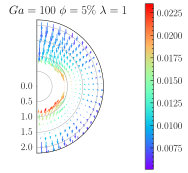
\includegraphics[height=0.35\textwidth]{image/HOMOGENEOUS_NEW/Dist/U_rel_l_1_Ga_100_PHI_5.pdf}
    % \begin{tikzpicture}[scale=0.8]
    %     \filldraw[ gray!50!white](0,0) circle (0.5);
    %     \filldraw[ gray!50!white](1,3)circle (0.5);
    %     \filldraw[ gray!50!white](-0.2,3.5)circle (0.5);
    %     % \draw[fill=gray,opacity=0.2](5,-0.2)circle (0.5);
    %     % \draw[fill=gray,opacity=0.2](-3,2)circle (0.5);
    %     % \draw[fill=gray,opacity=0.2](-5,0.2)circle (0.5);
    %     \draw(0,0)node[right]{$p_1, \; \textbf{x} = 0 $};
    %     \draw[dashed](0,0)--(1,3)node[right]{$p_2, \;\textbf{x}+\textbf{r}$};
    %     \draw[dashed](-0.2,3.5)node[right]{$p_3$};
    % \end{tikzpicture} 
    % \includegraphics[height=0.35\textwidth]{image/HOMOGENEOUS_NEW/Dist/U_rel_l_10_Ga_10_PHI_5.pdf}
    % 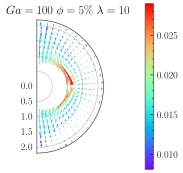
\includegraphics[height=0.35\textwidth]{image/HOMOGENEOUS_NEW/Dist/U_rel_l_10_Ga_100_PHI_5.pdf}
    \caption{
         Quiver plots of the relative averaged velocity field $\textbf{w}^\text{r}(\textbf{x},\textbf{r},t)$ colored by the averaged dimensionless age $a^r(\textbf{x},\textbf{r},t)$ for $\phi = 0.05$ and $\lambda +1$.
         (left) $Ga = 10$ (right) $Ga =100$. }
    \label{fig:Why_Ga_matter}
\end{figure}

The first aspect that we would like to clarify is the non-fore-aft symmetry of the velocity fields $\textbf{w}_p^\text{nst}$ with respect to the horizontal plane. 
% Indeed, in plots displayed on \ref{fig:Why_Ga_matter} we remark that the $\textbf{w}_p^\text{nst}$ exhibit a clear asymmetry with respect to the horizontal plane.
This is explained by the non commutativity of the function $h_{ij}$ in the indices $i$ and $j$ in \ref{eq:q_nstij}, as a result $\textbf{w}_p^r(\textbf{x},t,r,\theta) \neq \textbf{w}_p^r(\textbf{x},t,r,-\theta)$. 
Indeed, as it is depicted on \ref{fig:diagram_asym}, in the cases where the neighboring nearest droplet is far from the test droplet, the chance for this droplet to have another nearest neighbor which is closer is high. 
Thus, the nearest neighbor of the nearest neighbor of the test droplet, is not necessarily the test droplet. 
This induces an asymmetry in the nearest neighbor statistics. 
That explains why the plots on \ref{fig:Why_Ga_matter} are not symmetric when we observe the fields at sufficiently large distance $|\textbf{r}|$. 
Note that this asymmetry would not be present if we had considered classical particle pair average as done in \cite{shajahan2023inertial}. 

To summarize, in the situation where we observe $\textbf{w}_p^r$ for large $|\textbf{r}|$ the test droplet can be considered as being \textit{isolated}, as its nearest neighbor is at a large distance $|\textbf{r}|$ from the test droplet. 
Additionally, the nearest neighboring droplet, if located far enough, has 
potentially a nearest neighbor that is closer than the test sphere, as explained on \ref{fig:diagram_asym}. 
Consequently, provided that the nearest neighbor of the test sphere is far enough, we can be sure that on average it approaches a pair of droplets or more, that are packed together. 

\begin{figure}[h!]
    \centering
    \hfill
    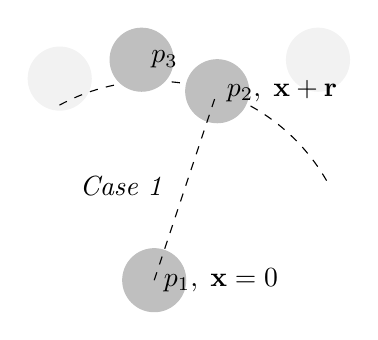
\begin{tikzpicture}[scale=0.8]
        \filldraw[ gray!10!white](+2.6,3.5)circle (0.5);
        \filldraw[ gray!10!white](-1.5,3.2)circle (0.5);
        \draw[dashed](30:3.16) arc (30:120:3.16);
        \filldraw[ gray!50!white](0,0) circle (0.5);
        \filldraw[ gray!50!white](1,3)circle (0.5);
        \filldraw[ gray!50!white](-0.2,3.5)circle (0.5);
        \draw(0,0)node[right]{$p_1, \; \textbf{x} = 0 $};
        \draw[dashed](0,0)--(1,3)node[right]{$p_2, \;\textbf{x}+\textbf{r}$};
        \draw[dashed](-0.2,3.5)node[right]{$p_3$};
        \node[ultra thick] (title) at (-0.5,1.5) {\textit{Case 1}};
    \end{tikzpicture} 
    \hfill
    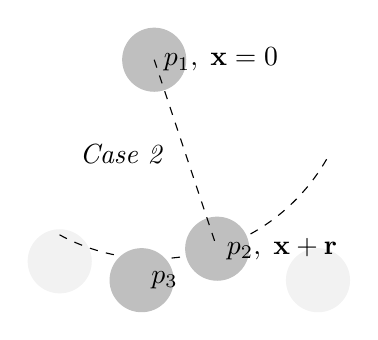
\begin{tikzpicture}[rotate=180, xscale=-0.8,yscale=0.8]
        \filldraw[ gray!10!white](+2.6,3.5)circle (0.5);
        \filldraw[ gray!10!white](-1.5,3.2)circle (0.5);
        \draw[dashed](30:3.16) arc (30:120:3.16);
        \filldraw[ gray!50!white](0,0) circle (0.5);
        \filldraw[ gray!50!white](1,3)circle (0.5);
        \filldraw[ gray!50!white](-0.2,3.5)circle (0.5);
        \draw(0,0)node[right]{$p_1, \; \textbf{x} = 0 $};
        \draw[dashed](0,0)--(1,3)node[right]{$p_2, \;\textbf{x}+\textbf{r}$};
        \draw[dashed](-0.2,3.5)node[right]{$p_3$};
        \node[ultra thick] (title) at (-0.5,1.5) {\textit{Case 2}};
    \end{tikzpicture} 
    \hfill
    % \begin{tikzpicture}[scale=0.8]
    %     \filldraw[ gray!10!white](+2.6,3.5)circle (0.5);
    %     \filldraw[ gray!10!white](-1.5,3.2)circle (0.5);
    %     \draw[dashed](-30:3.16) arc (-30:-120:3.16);
    %     \filldraw[ gray!50!white](0,0) circle (0.5);
    %     \filldraw[ gray!50!white](1,-3)circle (0.5);
    %     % \filldraw[ gray!20!white](-1.4,-3.3)circle (0.5);
    %     \filldraw[ gray!50!white](-0.2,-3.5)circle (0.5);
    %     % \draw[fill=gray,opacity=0.2](5,-0.2)circle (0.5);
    %     % \draw[fill=gray,opacity=0.2](-3,2)circle (0.5);
    %     % \draw[fill=gray,opacity=0.2](-5,0.2)circle (0.5);
    %     \draw(0,0)node[right]{$p_1, \; \textbf{x} = 0 $};
    %     \draw[dashed](0,0)--(1,-3)node[right]{$p_2, \;\textbf{x}+\textbf{r}$};
    %     \draw[dashed](-0.2,-3.5)node[right]{$p_3$};
    %     \node[ultra thick] (title) at (-0.5,-1.5) {$Case\; 2$};
    % \end{tikzpicture} 
    \caption{
        Diagram that highlights the asymmetry of the nearest pair statistics when the nearest neighbor is relatively far from the test particle.
        (\textit{Case 1}) droplet $p_1$ with  its nearest neighbor, $p_2$, located at the \underline{top} of it. 
        (\textit{Case 2}) droplet $p_1$ with  its nearest neighbor, $p_2$, located at the \underline{bottom} of it. 
        (\textit{Case 1} and \textit{2})
        In these situations, the droplet $p_2$ located at $\textbf{x} + \textbf{r}$, is the nearest neighbor of the droplet $p_1$ located at $\textbf{x}$. 
        Since $|\textbf{r}|/d$ is assumed to be large, the nearest neighbor of the droplet $p_2$ is more likely to be another nearest neighbor than $p_1$ such as the droplet $p_3$, which is closer.
        This is due to the rapid decay of $P_\text{nst}$ for large $|\textbf{r}|/d$, see \ref{fig:Pnst_high_Ga}. 
        In these cases, the nearest neighbor of $p_1$ is $p_2$, but the contrary is not true, inducing asymmetry in the statistics.  
    }
    \label{fig:diagram_asym}
\end{figure}

Now that this issue has been clarified, we can proceed to interpret the plots in \ref{fig:Why_Ga_matter}.
The beginning of the interactions happens at the early ages, meaning in the dark blue areas in  \ref{fig:Why_Ga_matter}, which are located on the top or bottom of the droplet of reference.
The ending of the interactions corresponds to the greater ages, which are represented by the red areas. 
As shown by \ref{fig:Why_Ga_matter} (left), at low \textit{Galileo} number the nearest droplet has a tendency to come from the top or bottom and leave through the sides. 
If the nearest droplet is at a reasonable distance $|\textbf{r}| < 1.5d$ on the sides of the test droplet, we can see that the vertical relative velocity is on average zero, but positive in the radial component.
In this area, the age is at its maximum (dark red zone), therefore the interactions come to an end, meaning that the nearest droplets get replaced by another. 
Note that the droplets at a larger distance of the test droplet, say $|\textbf{r}|>2$, have an averaged positive vertical relative velocity. 
As discussed above, in this situation the neighbor on the side is more likely to be closer to another droplet. 
Consequently, if the test droplet is isolated, with neighboring droplets sufficiently far on the side, it will rise on average with a lower velocity than the latter droplets.
Thus, droplets at contact seem to get apart because of the non-zero radial velocity, and droplets at a distance seem to get apart because of the non-zero vertical velocity.  
Consequently, on average the side-by-side configuration is not stable in this case, which partly explains why the droplet distribution doesn't form any layer or such oriented microstructure at these $Ga$.   

% A plausible explanation for this phenomenon is that the leading droplet accelerate the trailing droplet with its wake on a first stage. 
% Then, the trailing droplet arise to the same altitude as the leading droplet, but still goes faster than the leading droplet due to the acceleration provided by the wake of the latter droplet.
% If the droplets get in contact then the interaction duration seem to last longer, and the droplets might even get trap in a small stagnation zone on the side of the droplets.


For high \textit{Galileo} numbers, see \ref{fig:Why_Ga_matter} (right), the relative averaged velocity is nearly zero on the sides and below the test droplet. 
It is a statistical representation, meaning that, $\textbf{w}_p^r = 0$, indicates that the droplets relative  velocities are not correlated with the relative position in this area. 
Thus, it is hard to say if the area where $\textbf{w}_p^r = 0$ corresponds to actual stagnation zones where both droplets are in equilibrium, or if the relative velocity is just not correlated. 

The droplets at a large distance on the top of the test droplet have a downward velocity. 
This means that if the test sphere is isolated and approaches one or several  droplets on top of it (see \ref{fig:diagram_asym} (\textit{Case 1})), it will eventually catch up the latter droplets. 
On the contrary, if the droplet is isolated and the nearest neighbor is at the bottom (see \ref{fig:diagram_asym} (\textit{Case 2})), the velocity is either pointing downward, or it is not correlated with the position, as indicated by the magnitude of $\textbf{w}_p^r$. 
A plausible explanation for this phenomenon is that the reference droplet, when being isolated, goes faster than the potentially packed nearest neighbor.
Therefore, the test sphere can either catch up with the nearest droplet if it is above, or move further away from it if it is below.
Also, it is interesting to note that in this case the droplets at near contact on the bottom of the test droplet result from early interaction, denoted by the dark blue zone. 
It can be interpreted as follows: since 
initial duration of interaction is on average low in this zone, it does mean that droplets replace an old nearest neighbor that were at near contact with the test droplets. 
Thus, in this case, the nearest neighbor reaches the test sphere which was rising slowly because of a potentially closer neighbor. 

Ultimately, the fields $\textbf{w}^r_p(\textbf{x},\textbf{r}, a)$ provide a quantitative averaged representation of what is known as the \textit{Drafting Kissing Tumbling} \citep{fortes1987nonlinear} mechanism. 
Indeed, in both cases droplets eventually approach vertically (\textit{Drafting}), nearly touch each other (\textit{Kissing}), and leave through the sides (\textit{Tumbling}). 
Statistically, the \textit{Tumbling} part is not present in the high inertia case, which explains the creation of anisotropic structures or more stable side-by-side configurations. 
For bubble pair interactions \citet{zhang2021three} observed such DKT behavior.
They also reported side-by-side stable configurations of pairs. 
However, at the same \textit{Galileo} as \citet{zhang2021three} ($Ga = 10$) we were not able to identify this mechanism. 


To support the observations made above, we displayed in \ref{fig:unst_ga} the absolute conditioned averaged center of mass velocity of the test sphere, defined as,
\begin{equation*}
    \textbf{u}^\text{r}_p(\textbf{x},\textbf{r},t)  
    =
    \frac{1}{P_r(\textbf{x},\textbf{r},t)}
    \int_0^\infty \textbf{u}^\text{nst}_pP_\text{nst}(\textbf{x},\textbf{r},t,a) da
\end{equation*}
In \ref{fig:unst_ga} (left) we see that the magnitude of the test droplet's vertical velocity is higher than the droplet phase vertical velocity $\textbf{u}_p$ when the nearest neighbor is at near contact to the test droplet, either above or below.
\begin{figure}[h!]
    \centering
    \includegraphics[height=0.35\textwidth]{image/HOMOGENEOUS_NEW/Dist/U_l_1_Ga_10_PHI_5.pdf}
    \includegraphics[height=0.35\textwidth]{image/HOMOGENEOUS_NEW/Dist/U_l_1_Ga_100_PHI_5.pdf}
    \caption{
         Quiver plots of the conditioned droplet velocity field $\textbf{u}^\text{r}(\textbf{x},\textbf{r},t)$ colored by the averaged dimensionless vertical velocity difference : $(\textbf{u}^\text{r} - \textbf{u}_p )/ \textbf{u}_p$, for $\lambda = 1$ and $\phi = 0.05$. 
         (left) Low \textit{Galileo} number $Ga = 10$.
        (right) High \textit{Galileo} number $Ga = 100$.
         }
    \label{fig:unst_ga}
\end{figure}
When the nearest neighbor is at a large distance from the test droplet, its average velocity is lower than $\textbf{u}_p$. 
When inertia is high, however, the test droplet velocity is higher when being isolated than with its neighbor at near contact. 
Additionally, we can see that when the droplet is on the side at near contact or below, the test sphere's velocity  is lower than the mean. 
In brief in the case of $Ga = 10$ it seems that isolated droplets rise slower than close neighbors packed together. 
While at higher \textit{Galileo} number it is the opposite, we observe that isolated droplets go faster than packed neighbors. 


\subsubsection{The volume fraction dependency}
As observed in \ref{fig:A} the effect of increasing $\phi$ is that it makes the droplet distribution slightly more isotropic for $\phi >0.1$. 
\begin{figure}[h!]
    \centering
    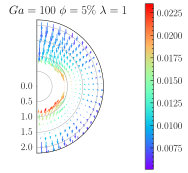
\includegraphics[height=0.35\textwidth]{image/HOMOGENEOUS_NEW/Dist/U_rel_l_1_Ga_100_PHI_5.pdf}
    \includegraphics[height=0.35\textwidth]{image/HOMOGENEOUS_NEW/Dist/U_rel_l_1_Ga_100_PHI_20.pdf}
    % \includegraphics[height=0.35\textwidth]{image/HOMOGENEOUS_NEW/Dist/U_rel_l_10_Ga_100_PHI_10.pdf}
    % \includegraphics[height=0.35\textwidth]{image/HOMOGENEOUS_NEW/Dist/U_rel_l_1_Ga_100_PHI_10.pdf}
    \caption{Quiver plots of the relative averaged velocity field $\textbf{w}^\text{r}(\textbf{x},\textbf{r},t)$ colored by the averaged dimensionless age $a^r(\textbf{x},\textbf{r},t)$, for $Ga = 100$ and $\lambda = 1$. 
    (left) Low \textit{Galileo} number $\phi = 0.05$.
    (right) High \textit{Galileo} number $\phi = 0.2$. }
    \label{fig:Why_Phi_matter}
\end{figure}
In \ref{fig:Why_Phi_matter} we expose two situations with various volume fractions. 
In both graphs, we observe the same trend, despite the changes in length scales, which are due to the variations in volume fraction. 
Indeed, the stagnation zones with dark red color and the droplet having short ages, dark blue color, are located approximately at the same location. 
We still observe the fore-aft asymmetry with respect to the horizontal plane, as was discussed above. 
For other $\lambda$ and $Ga$ no particular differences can be observed with varying $\phi$. 
Overall, even if small differences may be present, the change in volume fraction doesn't seem to affect the relative kinematics   of interaction between droplets. 

\subsubsection{Influence of the viscosity ratio}

Lastly, we turn our attention to the effect of the viscosity ratio on pair relative kinematics. 
The question that we are trying to answer is : why does a smaller viscosity ratio increase the anisotropy of the tensor $\textbf{R}(\textbf{x},t)$ as shown in \ref{fig:A}. 
With this objective in mind, we compare two cases at $Ga = 100$ and $\phi =0.05$, where we observe a clear difference between the distributions (see \ref{fig:Pnst_high_Ga}) between $\lambda = 1$ and $\lambda = 10$.
\begin{figure}[h!]
    \centering
    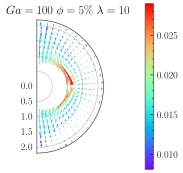
\includegraphics[height=0.35\textwidth]{image/HOMOGENEOUS_NEW/Dist/U_rel_l_10_Ga_100_PHI_5.pdf}
    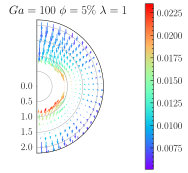
\includegraphics[height=0.35\textwidth]{image/HOMOGENEOUS_NEW/Dist/U_rel_l_1_Ga_100_PHI_5.pdf}
    % 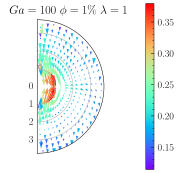
\includegraphics[height=0.35\textwidth]{image/HOMOGENEOUS_NEW/Dist/U_rel_l_1_Ga_100_PHI_1.pdf}
    % 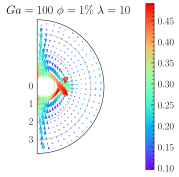
\includegraphics[height=0.35\textwidth]{image/HOMOGENEOUS_NEW/Dist/U_rel_l_10_Ga_100_PHI_1.pdf}
    \caption{Quiver plots of the relative averaged velocity field $\textbf{w}^\text{r}(\textbf{x},\textbf{r},t)$ colored by the averaged dimensionless age $a^r(\textbf{x},\textbf{r},t)$, for $\phi = 0.05$ and $Ga = 100$. 
    (left) High viscosity ratio $\lambda = 10$.
    (right) Low viscosity ratio, $\lambda = 1$. }
    \label{fig:Why_l_matter}
\end{figure}
As in the previous cases, it is clear that, for both cases in \ref{fig:Why_l_matter}, the neighboring droplet approaches on the vertical direction and ends its course on the sides.
As discussed previously, the case on \ref{fig:Why_l_matter} (right) exhibits a clear stagnation zone and asymmetry on a vertical plane. 
On the other hand for $\lambda =10$ the relative velocity in the vicinity of the droplet seems to be on average positive in the radial direction. 
In addition, The asymmetry aforementioned is not present in this case. 
As discussed in the previous paragraph, and explained by \ref{fig:diagram_asym}, the presence of the skew-asymmetry in the fields $\textbf{w}_p^\text{r}$ about the horizontal plane, is a sign of interactions of the isolated droplets with clusters of droplets.
The absence of such asymmetry implies the absence of such interactions, indicating that the droplets are more evenly spread. 

As before, it is interesting to investigate the value of the conditional velocity $\textbf{u}^r_p$ to better understand the droplets' collective interactions. 
Thus, \ref{fig:unst_l} display the fields  $\textbf{u}_p^\text{r}$ for both cases. 
\begin{figure}[h!]
    \centering
    \includegraphics[height=0.35\textwidth]{image/HOMOGENEOUS_NEW/Dist/U_l_10_Ga_100_PHI_5.pdf}
    \includegraphics[height=0.35\textwidth]{image/HOMOGENEOUS_NEW/Dist/U_l_1_Ga_100_PHI_5.pdf}
    \caption{
         Quiver plots of the conditioned droplet velocity field $\textbf{u}^\text{r}(\textbf{x},\textbf{r},t)$ colored by the averaged dimensionless vertical velocity difference : $(\textbf{u}^\text{r}_p - \textbf{u}_p )/ \textbf{u}_p$, for $\phi = 0.05$ and $Ga = 100$. 
         (left) High viscosity ratio $\lambda = 10$.
         (right) Low viscosity ratio, $\lambda = 1$.
         }
    \label{fig:unst_l}
\end{figure}
On \ref{fig:unst_l} (left) we first note that $\textbf{u}^\text{r}(\textbf{x},\textbf{r},t)$ behave similarly to the low inertia case displayed on \ref{fig:unst_ga} (left).
However, for $\lambda = 10$, the isolated droplets' velocity is roughly equal to $\textbf{u}_p$. 
Note that the trace of \textbf{R} is rather high in this case, (see \ref{fig:A}). 
Thus, the majority of the droplets are rather isolated. 
Consequently, if the isolated droplets rise at the average velocity of the dispersed phase it is because most of them are isolated droplets.
Therefore, this fact is not particularly relevant as it is just a statistical bias. 
Nevertheless, we can still conclude that for $\lambda = 10$ droplets go faster with a nearest neighbor on top or bottom, while for  $\lambda = 1$ droplets go faster when the nearest neighbor is at a large distance. 

\subsubsection{Relation with the dispersed phase velocity fluctuation tensor}

In addition to providing physical explanations, the field $\textbf{u}_p^d = \textbf{u}^r_p - \textbf{u}_p$ is of great importance to study the droplet phase fluctuation tensor $\pavg{\textbf{u}_i' \textbf{u}_i'}$ which is of crucial importance in multiphase flow modeling. 
Indeed, it can be shown that 
\begin{equation}
    \frac{\pavg{ \textbf{u}_i' \textbf{u}_i'}}{n_p}(\textbf{x},t)
    =  
    \int_{\mathbb{R}^3 }
    \textbf{u}_p^d
    \textbf{u}_p^d
    P_{nst}(\textbf{r}|\textbf{x},t)
    d\textbf{r}
    + \int_{\mathbb{R}^3 }
    \textbf{F}(\textbf{r},\textbf{x},t)
    d\textbf{r}
    \label{eq:particle_center_of_mass_velocities}
\end{equation}
where, $\textbf{F} = \avg{\sum_i\sum_{j\neq i}\delta_j\delta_i h_{ij}(\textbf{u}_i - \textbf{u}_p^{nst})(\textbf{u}_i - \textbf{u}_p^{nst})}$. 
Thus, the ensemble-averaged dispersed phase Reynolds stress is the sum of the fluctuation given by $\textbf{u}_p^r$ plus an additional contribution from the other droplet velocity fluctuations around the average field $\textbf{u}_p^d$. 
At low volume fraction, it is reasonable to think that the former term represents the majority of the droplet phase fluctuation.\footnote{
    However, note that it is note true in Stokes regime as the contribution from the second, third \ldots nearest droplets will become non-negligible even in the dilute regime. 
} 
Therefore, \ref{fig:unst_l} constitutes a visual representation of the droplet phase agitation tensor $\avg{\delta_i \textbf{u}_i' \textbf{u}_i'}$. 
Notably, we can remark on \ref{fig:unst_l}  that the droplet phase fluctuations tensor seems to be anisotropic. 
Indeed, more vertical velocity fluctuations than horizontal one is observed. 
This implies that the ``granular temperature'' $k_p = \pavg{ \textbf{u}_i' \cdot \textbf{u}_i'}/(2n_p)$ is probably not sufficient to model $\avg{\delta_i \textbf{u}_i' \textbf{u}_i'}$ in buoyant emulsions. 

Based on \ref{eq:particle_center_of_mass_velocities} we can compute the variance of the velocity of sedimenting suspensions of spherical droplets in Stokes and dilute regimes.
The method is quite similar than what is done in \citet{zhang2021ensemble} and \ref{chap:pseudoturbulence}. 
This idea will be pursued in a future study. 


\subsubsection{Discussion}
% \tb{
%     The field $\textbf{w}_p^r$ is useful for several reasons. 
%     As discussed it might serve to close equations such as \ref{eq:dt_R}. 
%     Or simply it provides us with clear physical explanation of what particles interaction look like. 
%     Also, we believe that it might be useful for coalesce kernels modeling. 

    
% }

From \ref{sec:Theory} we demonstrated that $\textbf{R}(\textbf{x},t)$ follows a transport equation where the tensor $\textbf{W}(\textbf{x},t)$ acts as a source term. 
This tensor might be expressed as the symmetric part of $\int_0^\infty \textbf{r} \textbf{w}_p^\text{r} P(\textbf{x},\textbf{r},t) da$. 
Thus, the trends of the $\textbf{w}_p^\text{r}(\textbf{x},\textbf{r},t) $ in terms of the position determine the value of $\textbf{W}(\textbf{x},t)$ and partly determine the final value of $\textbf{R}(\textbf{x},t)$. 
In many of the graphs, we observed that the vertical components of $\textbf{w}_p^\text{r}$ were negative when the vertical component of \textbf{r} was positive and vice versa. 
Consequently, $W_{yy}$ must be on average negative and $W_{xx}$ positive,this et  which ultimately contributes to the value of $\textbf{R}(\textbf{x},t)$ and $\textbf{A}(\textbf{x},t)$ through \ref{eq:dt_R} and justifies the sign of $A_{xx}$ in \ref{fig:A}. 

In \ref{fig:phase} we display the values of $W_{xx}$ in terms of $Ga$ and $\phi$. 
These graphs provide us with a concise description of the relative kinematics. 
We recall that $\textbf{W}:\bm\delta = 0$ as we demonstrated in \ref{sec:Theory}, thus the value  $W_{xx}$ entirely determines $W_{yy}$ since the problem is symmetric. 
For example, we see that the highest dimensionless relative velocity position is reached for $Ga = 10$ and $\phi = 0.01$. 
This implies that, it is in the dilute regime and with relatively small inertial effects, that the particles have the fastest relative motions. 
\begin{figure}[h!]
    \centering
    % \begin{tikzpicture}[scale=0.8]
    %     \node (img) at (0,0) {\includegraphics[height=5.5cm]{image/HOMOGENEOUS_NEW/PA/phase_Wxx_l_1.pdf}};
    %     \node (img) at (11,0) {\includegraphics[height=5.5cm]{image/HOMOGENEOUS_NEW/PA/phase_Wxx_l_10.pdf}};
    % \end{tikzpicture}
    \includegraphics[height=5.5cm]{image/HOMOGENEOUS_NEW/PA/phase_Wxx_l_1.pdf}
    \includegraphics[height=5.5cm]{image/HOMOGENEOUS_NEW/PA/phase_Wxx_l_10.pdf}
    \caption{Phase diagram of the horizontal components of the dimensionless correlation tensor $W_{xx}/(Ud)$. 
        (left) Iso-viscous emulsion $\lambda = 1$.
        (right) Viscous droplets $\lambda = 10$ }
    \label{fig:phase}
\end{figure}
Is the relative velocity fields $\textbf{w}_p^r$ the cause of the microstructure shape as is suggested by \ref{eq:dt_R}. 
Or does $\textbf{w}_p^r$ the consequence of microstructure shape? 
As suggested by the previous graphs \eqref{fig:Why_Ga_matter,fig:Why_l_matter,fig:Why_Phi_matter}. 
Indeed, on \ref{fig:Why_l_matter} (right), the clear asymmetry with respect to the horizontal plane can be explained as the consequence of clusters in the flows. 
Although it is a complicated question, we believe that both are true, even if physical parameters also impact $\textbf{w}_p^r$, which makes the microstructure case dependent.  
Nevertheless, this makes $\textbf{W}(\textbf{x},t)$ potentially a function of $\textbf{R}(\textbf{x},t)$.
Depending on its relationship with $\textbf{R}(\textbf{x},t)$ this may modify the relaxation time.  
Thus, a more efficient way to close \textbf{W} in an objective manner would be to study the dynamic of interactions. 
In this work, we only provided kinematics   arguments to explain the microstructure shape. 
Of course to fully understand the physics of interaction one has to study the dynamics of interactions. 
It is in fact possible in our framework to include such dynamics variable by deriving an equation for \textbf{W} the same way we derived \ref{eq:dt_R} for \textbf{R}.
Thus work is still needed to fully understand interaction dynamics within this ``nearest-particle statistics'' framework. 




% \subsection{Carrier phase velocity fields}

In the previous section we explained the microstructure formation with kinematic arguments.
Although we indeed provided an explanation the question that arise now id :
Why does the relative velocity behave as such.
The answer might be obtained based on dynamical arguments as it is done often, in such a way we could explain the relative kinematic.
Nevertheless, the dynamical aspect of the interaction is out of the scope of this study and will be treated in a future work. 

Instead, we propose to study the particles averaged wakes to explain the possible difference in interaction between the iso-viscous and viscous droplets cases. 
Again we make use of the nearest particle averaged statistic to compute the carrier fluid phase velocity conditionally on the presence of a particle at \textbf{x}, it reads,
\begin{equation*}
    \textbf{u}^\text{nst}_f P_{nst}(\textbf{x},\textbf{r},t)= 
    \int \sum_{i}^{N_b} \delta(\textbf{x}-\textbf{x}_i(\FF,t))
    h_{i} 
    \textbf{u}_f^0(\textbf{x}+\textbf{r},t,\FF)
    d\mathscr{P} 
\end{equation*}
where $h_{i} = 1$ if the particle $i$ center of mass is the nearest point to the eularian coordinate \textbf{x}+\textbf{r}. 
This velocity fields can be reconstructed as well with our DNS. 
On \ref{fig:stream} we display the reconstructed velocity field $\textbf{u}^\text{nst}_f$ for (left) the iso-viscous case $\lambda =1$ and (right) the viscous droplets' case $\lambda = 10$, for different value of the volume fraction. 
\begin{figure}[h!]
    \centering
    \includegraphics[height=0.4\textwidth]{image/HOMOGENEOUS_NEW/Stream/Stream_PHI_1_Ga_100_l_100}
    \includegraphics[height=0.4\textwidth]{image/HOMOGENEOUS_NEW/Stream/Stream_PHI_1_Ga_100_l_10}
    \includegraphics[height=0.4\textwidth]{image/HOMOGENEOUS_NEW/Stream/Stream_PHI_5_Ga_5_l_100}
    \includegraphics[height=0.4\textwidth]{image/HOMOGENEOUS_NEW/Stream/Stream_PHI_5_Ga_5_l_10}
    \includegraphics[height=0.4\textwidth]{image/HOMOGENEOUS_NEW/Stream/Stream_PHI_20_Ga_100_l_100}
    \includegraphics[height=0.4\textwidth]{image/HOMOGENEOUS_NEW/Stream/Stream_PHI_20_Ga_100_l_10}
    % \includegraphics{image/HOMOGENEOUS_NEW/Stream/Stream_PHI_5_Ga_100_l_1.pdf}
    \caption{Nearest averaged carrier phase velocity fields. }
    \label{fig:stream}
\end{figure}
This velocity field is evaluated at $\textbf{x}+\textbf{r}$ conditioned on the presence of the nearest particle at $\textbf{x}$. 


\tb{compare with \citet{shajahan2023inertial} for explaination }

\section{Conclusion}
\section{Conclusion}

% \citet{einstein1905neue,taylor1932viscosity} demonstrated how the first moment of the hydrodynamic forces (Stresslet) applied on a particle immersed in pure linear flow induced an additional viscosity to the mixture. 
% Later~\citet{zhang1994ensemble,lhuillier1996contribution,jackson1997locally,zhang1997momentum} demonstrated that the second moment of forces were also contributing to the stresses inducing a non-newtonian behaviors, even in the Stokes and dilute limit.  

In this work we computed the moments of force on the surface of a test droplet in the situation of uniform relative motions between the droplet and the continuous phase. 
We considered low but finite Reynolds number $Re$. 
The averaged first moment of force is given by~\ref{eq:forces_reformulated2_avg}, scales as $O(\rho_f \phi u_r^2)$, hence contributing to the averaged Stress of the suspension on the same ground as  \citet{einstein1905neue} or \citep{taylor1932viscosity} correction to the viscosity of the mixture. 
In a lesser extend the inertial part of the second moment also contribute to the Rheology. 
This first point constitutes the main result of the paper. 

Others important conclusion reached through this work includes: a general reciprocal formula to derive the forces and moments on droplets, and the explicit appearing of the velocity variance term in the drag force term. 







\appendix

\section{Numerical validations}
\label{ap:validation}

The \texttt{Basilisk} code has been validated numerous time in previous numerical studies. 
Especially, we can cite the recent studies of \citet{innocenti2020direct} and \citet{hidman2023assessing} which both performed DNS of rising suspension of bubbles. 
Nevertheless, in this work we investigate specific statistical distribution,
and we make use of a multi-VoF method to avoid droplets coalescence, therefore a meticulous validation of the DNS is in order. 
We start by presenting a brief comparison with the reference DNS \citet{esmaeeli1999direct}. 
Afterward we present a study focusing on the interfaces' kinematic, we compare our DNS with the experimental results of \citet{mohamed2003drop} in the objective to show that the Multi-VoF method indeed capture the physics of two colliding interfaces without solving the flows in the film. 
Once the mesh and the physics are validated, a study on the convergence of the statistics is presented. 

\subsection*{Ordered array of buoyant bubbles}

From our knowledge, no simulations nor experimental results have been carried out for rising buoyant viscous drop. 
Therefore, instead we reproduced the ordered array simulation of \citet{esmaeeli1999direct} with \texttt{Basilisk} to validate the mesh definition of our DNS.  
It consists in a 3-D buoyant ordered rising array of bubbles. 
In our notation the flow parameters of the simulation reads, 
\begin{align*}
    \lambda = 10,
    && \zeta = 10,
    && Bo = 1.8,
    && Ga = 28.37,
    && \phi = 0.125.
\end{align*}
\begin{figure}[h!]
    \centering
    \includegraphics[height = 0.3\textwidth]{image/VALIDATION2.0/Loisy/Re.pdf}
    \caption{Time evolution of the Reynolds number based on the instantaneous volume averaged drift velocity, $Re(t) = \rho_fU d /\mu_f$, with $U(t) = |\textbf{u}_p - \textbf{u}_f|$ with $\phi = 0.1256$, $\zeta =\mu_r =10$ and $Ga = 29.9$.
    $\textbf{u}_p$ and $\textbf{u}_f$ are the particle and fluid phase volume averaged velocity at time $t$.}
    \label{fig:ordered_array}
\end{figure}
\ref{fig:ordered_array} display our numerical simulation against the original result of \citet{esmaeeli1999direct}.
We observe very good agreements between both studies for all mesh definition.
Additionally, we displayed the results of \citet{innocenti2020direct} for $d/\Delta = 20$ to point out a divergence with our results at the same mesh definition.  
Both our simulations and the one of \citet{innocenti2020direct} have been carried out with the  \texttt{Basilisk} code. 
The cause of this difference is in fact due to a different method of interpolation used for the viscosity coefficient $\mu$. 
We used an arithmetic mean, whereas \citet{innocenti2020direct} used a 
harmonic mean.
As a matter of fact in this regime the arithmetic mean, which will be used in this work, permit us to reach a faster convergence. 
Overall these results indicate that the criterion $d/\Delta = 30$ seems sufficient, which is consistent with the aforementioned studies.


\subsection*{Drop impact on a liquid-liquid interface}

In section, we investigate in more detail the physics behind the Multi-VoF method. 
We need to verify if we accurately capture the physics of the droplets interfaces despite the fact that we do not model accurately  the film between two droplets. 
Following \citet{balcazar2015multiple} we reproduced the experiment of drop impact on a liquid–liquid interface carried by \citet{mohamed2003drop} but with the \texttt{Basilisk} code. 
This experiment consist in letting a drop fall into a pool of the same fluid as the drop, all along the experiment the interfaces of the droplets and the pool are tracked. 
In our notation the dimensionless parameters of latter study reads, 
\begin{align*}
    Ga = 71.02 
    && Bo = 6.40
    && \lambda = 0.33
    && \zeta = 1.189
\end{align*}
Following \citet{mohamed2003drop} we defined the dimensionless time $t / t_i = t U_i(t) /d$ where $U_i(t)$ is droplet velocity at $t<0$ and where $t=0$ is the time of impact. 
Regarding the geometry of the problem we sketched in \ref{fig:schemeLong} a scheme of the initial position of the droplet in the computational domain.
Additionally, we displayed on \ref{fig:schemeLong} a snapshot of the numerical domain were we see the drop colliding the pool's interface.
Both, the drop and the pool does not merge since we use the Multi-VoF method, note that in the experiment the drop does not merge with the pool either.
This enables us to represent with DNS a physical situation where the interfaces do not coalesce, but where we use a grid definition of $d/\Delta = 30$ which is of course not sufficient to model the flow inside the film. 
\begin{figure}[h!]
    \centering
    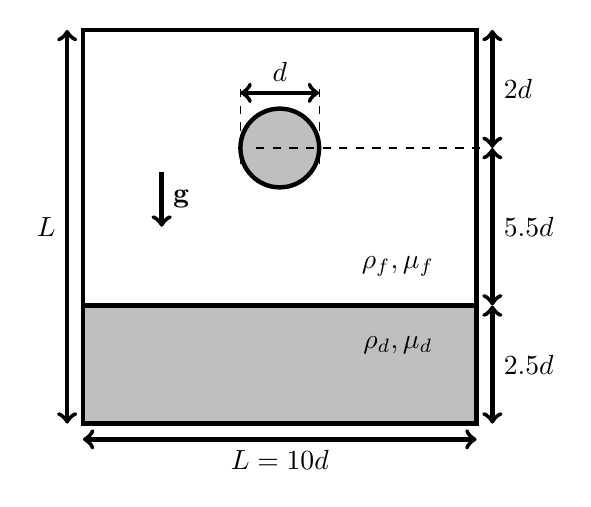
\begin{tikzpicture}[ultra thick]
        \draw (0,0) rectangle (5,5);
        \draw[fill=gray!50] (0,0) rectangle (5,1.5);
        \draw[fill=gray!50] (2.5,3.5) circle (0.5);
        \draw[<->](0,-0.2) --++ (5,0)node[midway,below]{$L  = 10 d$};
        \draw[<->](-0.2,0) --++ (0,5)node[midway,left]{$L$};
        \draw[<->](5.2,0) --++ (0,1.5)node[midway,right]{$2.5 d$};
        \draw[<->](5.2,1.5) --++ (0,2)node[midway,right]{$5.5 d$};
        \draw[<->](5.2,3.5) --++ (0,1.5)node[midway,right]{$ 2d$};
        \draw[dashed,thin](2.2,3.5) --++ (2.9,0);
        \draw[dashed,thin](2.2,3.5) --++ (2.9,0);
        \draw[->](1,3.2) --++ (0,-0.7)node[midway,right]{$\textbf{g}$};
        \draw[<->](2,4.2) --++ (1,0)node[midway,above]{$d$};
        \draw[thin,dashed](2,3.3) --++ (0,1);
        \draw[thin,dashed](3,3.3) --++ (0,1);
        \node (a) at (4,2){$\rho_f, \mu_f$};
        \node (a) at (4,1){$\rho_d, \mu_d$};
    \end{tikzpicture}
    \includegraphics[height = 0.4\textwidth]{image/VALIDATION2.0/Longmire/IMG/image-079.png}
    \caption{(left) Scheme of the computational set up at the initial time. 
    (right) Snapshot of the computational domain after the collision time, with the pool interfaces represented in gray.
    The background color represents the velocity field magnitude, which is undisturbed, indicating a large enough domain. }
    \label{fig:schemeLong}
\end{figure}
\begin{figure}[h!]
    \centering
    \includegraphics[height = 0.3\textwidth]{image/VALIDATION2.0/Longmire/Re.pdf}
    \includegraphics[height = 0.3\textwidth]{image/VALIDATION2.0/Longmire/Dist.pdf}
    \caption{(left) Time evolution of the Reynolds number based on the droplet velocity, $Re(t) = \rho_fU d /\mu_f$ in terms of the dimensionless time, (+) numerical results of  \citet{balcazar2015multiple} (right)  position of the interfaces, ($\bullet$) top droplets surface, ($+$) bot droplet surface, (x) pool surface. (Symbols) experimental result of \citet{mohamed2003drop} (solid line) present numerical simulations with $d/\Delta = 30$. }
    \label{fig:resultslong}
\end{figure}
\ref{fig:resultslong} represent the comparison between our results against the experiment of \citet{mohamed2003drop} (right) and the numerical simulation of \citet{balcazar2015multiple} (left). 
The time dependent Reynolds number as well as the interfaces positions are shown to match exactly both, the numerical and experiential results of \citet{balcazar2015multiple} and \citet{mohamed2003drop}, respectively. 
From the very good agreement obtained with the numerical and experimental results we conclude that the kinematic is preserved during the contact time for a mesh definition of $d/\Delta = 30$. 

\subsection*{Mesh independence and statistical convergence for random array of drops}

Even through aforementioned studies carried validation of the \texttt{Basilisk} code for rising droplets or bubbles, almost all of them considered isolated droplets or bubbles as the only validation case. 
As far as the author's knowledge, to this date no published study presented a mesh independence study for random array of droplets nor bubbles of this scale. 
Nevertheless, as particles interaction and higher \textit{Galileo} numbers may be more challenging to model, it is primordial to investigate the mesh independence of the exact same DNS that are carried in this work. 
In this objective we performed DNS of random array of $N_b=125$ droplets, with the following parameters,
\begin{align*}
    \lambda = 10,
    && \zeta = 1.11,
    && Bo = 1,
    && Ga = 100,
    && \phi = 0.1,
    && N_b =125,
\end{align*}
and the mesh definition is, $d/\Delta = 7.37, 14.74, 29.9 58.97$. 
We expect that the most challenging DNS simulated in this work is for the case, $\lambda = 10$ and $Ga = 100$, since it is in this range of parameters that we induce the most vorticity, which ultimately require good mesh definition. 
Additionally, in opposition to the ordered array case, this case includes droplets interaction, which ultimately induce more numerical complexities to tackles. 
Based on this remark we can assume that if this case is mesh independent, then all cases from \ref{tab:simulations} must be since this is the most challenging scenario.   

Let's first verify the independence of the drift velocity on the mesh definition. 
\begin{figure}[h!]
    \centering
    \includegraphics[height = 0.3\textwidth]{image/HOMOGENEOUS_NEW/VAL/Re.pdf}
    \caption{
        Running average of the Reynolds number based on the instantaneous volume averaged drift velocity, $Re(t) = \rho_fU d /\mu_f$, with $U(t) = |\textbf{u}_p - \textbf{u}_f|$ for $\phi = 0.1$, $Ga=100$ and $\lambda =10$.
        $\textbf{u}_p$ and $\textbf{u}_f$ are the particle and fluid phase volume averaged velocity at time $t$.
        In the legend we display the value of the mesh definition. 
    }
    \label{fig:Re}
\end{figure}
In \ref{fig:Re} we display the running averaged drift velocity in terms of time, for four mesh definition. 
The results are not as independent of the mesh definition as the order array validation presented above. 
Indeed, we observe a difference of the rising Reynolds number of about $5\%$ between the $d/\Delta = 29.49$ and $d/\Delta = 58.97$ cases which is notable.
We recall that this $5\%$ error will eventually be lower for all other cases. 
The good agreement between the case  $d/\Delta = 14.74$ and $d/\Delta = 29.49$ is partially fortuitous.

Now let's study the mesh influence on the statistics. 
It is clear from \ref{fig:apstat} (left) that both mesh definition produce nearly the same radial distribution, no notable difference is identified. 
In \ref{fig:apstat} (middle) we can observe the age distribution for both mesh definition. 
It is clear that refining the mesh induce a difference in the age distribution. 
As, a matter of fact it has a small impact on the mean age, $\tau_p = 6.96$ for the lower definition, and $\tau_p = 6.14$ for the finest grid.
This makes a $10\%$ error, but as mentioned above this is probably the highest error that we could encounter among all cases. 
\begin{figure}
    \centering
    \includegraphics[height = 0.24\textwidth]{image/HOMOGENEOUS_NEW/VAL/Pr.pdf}
    \includegraphics[height = 0.24\textwidth]{image/HOMOGENEOUS_NEW/VAL/Pa.pdf}
    \includegraphics[height = 0.24\textwidth]{image/HOMOGENEOUS_NEW/VAL/w.pdf}
    \caption{
        Statistical averaged functions for two mesh definition. 
        (left) Radial normalized probability density function  $P_r(\textbf{x},|\textbf{r}|,t)/P_\text{th}$, in terms of the dimensionless radial position. 
        (middle) Probability density function of the age distribution $P_a(\textbf{x},t,a)$. 
        (right) Nearest averaged dimensionless approach velocity for both mesh definition, in terms of the dimensionless age. 
    }
    \label{fig:apstat}
\end{figure}
Even through an error is identified on the mean age of interaction we still notice that both nearest averaged dimensionless approach velocity on \ref{fig:apstat} (right) match perfectly. 
\begin{figure}[h!]
    \centering
    \includegraphics[height = 0.3\textwidth]{image/HOMOGENEOUS_NEW/VAL/U_rel_ndc_25.pdf}
    \includegraphics[height = 0.3\textwidth]{image/HOMOGENEOUS_NEW/VAL/U_rel_ndc_35.pdf}
    \caption{Quiver plots of the relative averaged velocity field $\textbf{w}^\text{r}(\textbf{x},\textbf{r},t)$ colored by the averaged dimensionless age $a^r(\textbf{x},\textbf{r},t)$, for $\phi = 0.05$ and $Ga = 100$. 
    (left) Low mesh definition.
    (right) High mesh definition. 
    }
    \label{fig:velap}
\end{figure}
Regarding, the 2D fields  $\textbf{w}^\text{r}(\textbf{x},\textbf{r},t)$ we can see that no notable difference can be identified, if it is not the slight difference in the value of the age scale. 


Overall, the one dimensional and two-dimensional conditioned statistics are almost independent of the mesh definition. 
By obtaining the same statistics with two independent DNS makes us confident on the fact that our numerical samples is large enough.
Indeed, if the samples were not sufficient we would have obtained two different distribution functions, thus we can be sure that the statistics have well converged. 
The slight difference in rising velocity and age distribution found for these Reynolds number must be acknowledged.
As mentioned at the beginning, this case is in fact very challenging as the volume fraction of droplets is consequent which induce numerous inertial interactions. 
Nevertheless, we can be sure that our final results is accurate at most with a $5\%$ error for this case, and probably less for the others cases. 
These, error testify for the very challenging  aspect of these simulations. 
Overall, we have great confidence in the statistical and physical representativity of our DNS results. 
\section{Age distribution at low \textit{Galileo} numbers}
\label{ap:age}

We provide additional age distribution for low \textit{Galileo} number to support the argumentation in the body of the text. 
\begin{figure}[h!]
    \centering
    \includegraphics[height = 0.3\textwidth]{image/HOMOGENEOUS_NEW/Dist/Pa_l_1_Ga_10.pdf}
    \includegraphics[height = 0.3\textwidth]{image/HOMOGENEOUS_NEW/Dist/Pa_l_10_Ga_10.pdf}
    \caption{(left) Age distribution at $\lambda = 10$ and $Ga = 10$ for : (solid line) $\phi = 0.2$; (dash dotted line) $\phi = 0.1$; (dashed line) $\phi =0.05$; (dotted line) $\phi = 0.01$. 
    (right) Mean dimensionless age in terms of the volume fraction $\phi$ for : 
    ($\bullet$) $Ga=1$; ($\blacktriangle$) $ Ga = 10$; ($\blacksquare$) $Ga = 50$ ($\blacklozenge$) $Ga =100$.
    The age and $\tau_a$ are made dimensionless with $U/d$ where $U$ is the drift-velocity between the dispersed and continuous phase.  }
    \label{fig:age_picture}
\end{figure}

\bibliography{Bib/bib_bulles.bib}

\end{document}

